\pdfoutput=1
\documentclass[11pt,letter,subeqn,fleqn]{article}
\usepackage[normalem]{ulem}
\usepackage{amsmath, amssymb,amsthm,cite}
\usepackage[dvips]{graphics}
\usepackage[usenames,dvipsnames]{color}
%\usepackage[normal]{subfigure}
%\usepackage{subfig}
\usepackage{graphicx}
\usepackage{tabulary}
\usepackage{float}
\usepackage{gensymb}
\usepackage{authblk}
\usepackage{caption}
\usepackage{subcaption}
\usepackage{xcolor} % added by Shawn

\DeclareGraphicsExtensions{.pdf,.png,.jpg,.eps}
\usepackage{mathtools}
\DeclarePairedDelimiter{\abs}{\lvert}{\rvert}
\usepackage{epsfig}
\usepackage{latexsym}
\usepackage{amsmath}
\usepackage{amssymb}
\usepackage{mhsetup}
\usepackage{mathtools}
%\usepackage{mathrsfs}
%\usepackage{float}
\usepackage{xfrac}
\numberwithin{equation}{section}
\numberwithin{table}{section}
\numberwithin{figure}{section}
%\usepackage[round]{natbib}
\usepackage{epsfig}
\usepackage{epstopdf}
\usepackage{tabulary}
\usepackage{threeparttable}
\usepackage{array}
\usepackage{siunitx}
\usepackage{booktabs}
\usepackage{multirow}
\usepackage{pbox}
\usepackage{lipsum}
\usepackage{enumerate}
\usepackage{caption,setspace}
\captionsetup{font={large,stretch=1}}

\title{Nonlinear Love Wave Models in Hyperelasticity and Viscoelasticity Frameworks}

\author[1]{Samuel Opoku Agyemang \thanks{Electronic mail: soa964@usask.ca}}
\author[1]{Alexei Cheviakov\thanks{Corresponding Author. Alternative English spelling: Alexey Shevyakov. Electronic mail: alexei.cheviakov@usask.ca}}
\affil[1]{Department of Mathematics and Statistics, University of Saskatchewan}
%\affil[2]{Department of Mathematics and Statistics, University of Saskatchewan}


\setlength{\textwidth}{160.0mm} \setlength{\textheight}{240.0mm}
\setlength{\oddsidemargin}{6mm} \setlength{\evensidemargin}{0mm}
\setlength{\topmargin}{-28mm} \setlength{\parindent}{5.0mm} \setlength{\parskip}{1.0mm}


\tolerance=9999

\def \dfracskip{2ex}

\def\beq{\begin{equation}}
\def\eeq{\end{equation}}
\def\barr{\begin{array}{ll}}
\def\earr{\end{array}}
\def\eps{\varepsilon}

\def\sg#1{{\rm #1}}
\def\const{\hbox{\rm const}}
\def\diag{\hbox{\rm diag}}
\def\mod{\hbox{\rm mod}}
\def\rank{\mathop{\hbox{\rm rank}}}
\def\Image{\mathop{\hbox{\rm Image}}}
\def\mes{\mathop{\hbox{\rm mes}}}
%\def\grad{\mathop{\hbox{\rm grad}}}
\def\sign{\mathop{\hbox{\rm sign}}}
\def\ind{\mathop{\hbox{\rm ind}}}
\def\id{\mathop{\hbox{\rm id}}}
\def\d{\mathop{\hbox{\rm d}}}
\def\ad{\hbox{ad}}
\def\ch{\mathop{\hbox{\rm ch}}}
\def\th{\mathop{\hbox{\rm th}}}
\def\cth{\mathop{\hbox{\rm cth}}}
\def\sh{\mathop{\hbox{\rm sh}}}
\def\max{\mathop{\hbox{\rm max}}}
\def\ind{\mathop{\hbox{\rm ind}}}
\def\Tr{\mathop{\hbox{\rm Tr}}}
\def\grad{{\hbox{\rm grad}}}
\def\div{{\hbox{\rm div}}}
\def\Div{\mathop{\hbox{\rm Div}}}
\def\curl{\mathop{\hbox{\rm curl}}}
\def\sn{\mathop{\hbox{\rm sn}}}
\def\sech{\mathop{\hbox{\rm sech}}}
\def\vec#1{{\boldsymbol{\rm #1}}} %\def\vec#1{{\bf {#1}}}
\def\veci#1{{\boldsymbol{#1}}} %\def\vec#1{{\bf {#1}}}
\def\tens#1{{\boldsymbol{\rm #1}}} %\def\vec#1{{\bf {#1}}}
\def\p{\partial}
\def\cn{\mathop{\hbox{\rm cn}}}
\def\sn{\mathop{\hbox{\rm sn}}}
\def\dn{\mathop{\hbox{\rm dn}}}
\def\scn{\mathop{\hbox{\footnotesize\rm cn}}}
\def\ssn{\mathop{\hbox{\footnotesize\rm sn}}}
\def\sdn{\mathop{\hbox{\footnotesize \rm dn}}}
\def\vec#1{{\boldsymbol{\rm #1}}} %\def\vec#1{{\bf {#1}}}
\def\tens#1{{\boldsymbol{\rm #1}}} %\def\vec#1{{\bf {#1}}}



%%% One Parameter %%%
\newcommand{\norm}[1]{\|{#1}\|}

%%% Two Parameters %%%
\newcommand\der[2][]{\ensuremath{\frac{d#1}{d#2}}}
\newcommand\pder[2][]{\ensuremath{\dfrac{\partial #1}{\partial #2}}}
\newcommand\sder[2][]{\ensuremath{\dfrac{{d}^{2}#1}{{d#2}^{2}}}}
\newcommand\spder[2][]{\ensuremath{\dfrac{{\partial}^{2}#1}{{\partial#2}^{2}}}}
\newcommand\tpder[2][]{\ensuremath{\dfrac{{\partial}^{3}#1}{{\partial#2}^{3}}}}



\newtheorem{theorem}{Theorem}
\newtheorem{theoremp}{Principal Result}
\newtheorem{lemma}{Lemma}
\newtheorem{proposition}{Proposition}
\newtheorem{corollary}{Corollary}

{\theoremstyle{definition} \newtheorem{definition}{Definition}
\newtheorem{example}{Example}
\newtheorem{remark}{Remark}
}

%\newcommand{\vspacebefore}{\raisebox{0ex}[3.8ex][0ex]{\null}}
\newcommand{\vspacebefore}{\raisebox{0ex}[3.9ex][0ex]{\null}}


\newcounter{tabnum}\setcounter{tabnum}{0}
\renewcommand{\thefootnote}{\alph{footnote})}


\newcommand{\boldsig}{\mbox{\mathversion{bold}$\sigma$}}
\newcommand{\boldphi}{\mbox{\mathversion{bold}$\phi$}}

\newcommand{\boldsigma}{\mbox{\mathversion{bold}$\sigma$}}
%\newcommand{\boldphi}{\vec{\phi}}
\renewcommand{\div}{\mathrm{div}}
\newcommand{\D}{\mathrm{D}}
\newcommand{\E}{\mathrm{E}}
\newcommand{\R}{\mathrm{R}}
\newcommand{\X}{\mathrm{Y}}
\newcommand{\W}{\mathrm{W}}
\newcommand{\Y}{\mathrm{Y}}
\newcommand{\Z}{\mathrm{Z}}
\newcommand{\sysR}{\vec{R}}
\newcommand{\C}{\vec{C}}
\newcommand{\B}{\vec{B}}
\newcommand{\boldP}{\vec{P}}
\newcommand{\boldF}{\vec{F}}
\newcommand{\boldE}{\vec{E}}
\newcommand{\sgn}{\mathop{\mathrm{sgn}}}
\newcommand{\linop}{\mathrm{L}}



%\newtheorem{prop}{Proposition}[section]
%\newtheorem{thm}{Theorem}[section]
%\newtheorem{cor}{Corollary}[section]


\def\PDEs#1#2#3{{\boldsymbol{\rm #1}}\{#2\,; #3\} }
\def\PDEsr#1#2#3#4{{\bf #1^\mathrm{#2}}\{#3\,; #4\} } %superscript roman
\def\PDEsi#1#2#3#4{{\bf #1^\mathit{#2}}\{#3\,; #4\} } %superscript ital
\def\PDEssh#1{{\bf #1} } %short form- no vars

\begin{document}


\maketitle \numberwithin{equation}{section}
\maketitle \numberwithin{remark}{section}
\numberwithin{lemma}{section}
\numberwithin{proposition}{section}


%%%%%%%%%%%%%%%%%%%%%%%%%%%%%%%  ABSTRACT  %%%%%%%%%%%%%%%%%%%%%%%%%%%%%%
\begin{abstract}

The study of nonlinear shear waves propagating in elastic materials is fundamentally important in various areas of science and technology, including material sciences, seismology, geology, natural resource exploration, biological material research, and further medical applications. In the current contribution, the concept of Love waves, linear shear waves propagating in the ground as a result of an earthquake and having small displacements parallel to the ground surface, is generalized to the situation when the displacements are not small. A nonlinear wave partial differential equation (PDE) is derived, describing such displacements for an arbitrary incompressible hyperelastic material specified by a stored energy constitutive function. The hydrostatic pressure present in the model is explicitly found in terms of the stored energy.
As a further generalization, a new PDE describing a broad class of hyper-viscoelastic materials is obtained, involving mixed space-time third order derivatives of the displacement. The obtained models provide a more precise approximation of shear displacements as opposed to the linear Love wave framework.
\end{abstract}


%%%%%%%%%%%%%%%%%%%%%%%%%%%%% INTRODUCTION %%%%%%%%%%%%%%%%%%%%%%%%%%%%%%
\section{Introduction}


* Surface and volume waves are different (Wiki)

* Love/surf waves don't decay as fast with distance

* Love def: geo, mech.

* Wiki def: $u=w=0$,  $v\sim \exp(i(kx-\omega t))$ - harmonic

* Love: sol of the same hyperbolic-type wave eq as shear waves, just with diff BCs. Nodes, decay... We derive those eqs

* Discuss constitutive problem in Intro; refer to Hess and some fund works in thermoelast...

* Rename 1d reductions to bulk s-waves



Deeper understanding of the propagation of seismic waves is crucial for the study of various geological processes, including earthquakes and volcanic eruptions, as well as exploration of natural resource deposits in the Earth. The Earth's crust is highly non-homogeneous; different rock types in the crust exhibit different kinds of elastic and viscoelastic behavior. A displacement of material particles in a domain filled with an elastic material is described by the full set of nonlinear elasticity equations that have similar mathematical structure for a variety of media, from rocks to complex biological and man-mae materials; models differ mainly by parameters and constitutive functions [MarsHughes, Ciarlet...].

Small material displacements within the elastic motion of a medium are often represented as a superposition of primary and secondary body waves (known as P-waves and S-waves, with displacements, respectively, parallel and perpendicular to the propagation direction). In general, for finite, non-small displacements, linear superposition principle does not hold, and P- and S-waves represent particular solution of full three-dimensional elasticity equations.

Unlike body waves, surface waves that arise on surfaces of contact of different media, in particular, on the Earth surface, enjoy properties different from those of the corresponding body waves. In seismology, the two main elastic surface wave types are the Rayleigh waves,


wave
propagate in elastic materials,


The Earth's crust is highly anisotropic??? and non-homogeneous; different rock types in the crust exhibit different kinds of elastic and viscoelastic behavior. *** similar problems arise in the study of waves in other materials, including modern complex man-made materials and biological tissues [JF and refs therein]


Nowadays, the damage caused by earthquakes to lives and properties has raised notable concerns. Also, owing to the emergence of more and accurate seismic instruments for measuring more earthquakes, quakes are recorded almost everyday in the world. For these reasons, seismic waves (surface waves) have become an interesting study area. Models obtained in this area of seismology are solved numerically or analytically. Love surface waves have various applications in earthquake engineering and seismology. They are dispersive waves that travel along the interface of the elastic layers and elastic half-spaces with different elastic moduli \cite{rushchitsky2011theory,rushchitsky2014nonlinear}.
Love surface waves propagate horizontally and travel faster in a horizontal plane than in the vertical direction, and this is termed as seismic anisotropy. Typical Love wave speed in the ground ranges from 2 km/s to 5 km/s. Love waves are formed by the interaction of a free surface and a horizontally polarized SH waves, and they are the fastest surface waves compared to Rayleigh waves since they have higher velocities. Hence in seismology, Love waves arrive first to a seismograph before Rayleigh waves. They can be considered plane waves with low velocities along the surface of the Earth. Love waves may arise in an isotropic layer overlying an isotropic elastic half-space (when both the layer are  in welded contact) if and only if the phase velocities satisfy the condition
\begin{equation}\label{eq:a4}
v^1_{T}<v_\mathrm{Love}<v^2_{T},
\end{equation}
\noindent ***really? Check wiki etc.*** where $v_\mathrm{Love}$ denotes Love wave velocity, $v^1_{T}$ is the shear wave phase velocity in the elastic layer, and $v^2_{T}$ is the shear wave phase velocity in the elastic half-space (Figure~\ref{fig:Love-type displacement}).

****************************Samuel put a Love-wave type diagram************************
%\begin{figure}[h]
%	\centering
%	\includegraphics[width=5in, height=4in]{Shearsam.pdf}
%	\caption{Love wave-type displacements near the surface of an elastic material.}
%	\label{fig:Love-type displacement}
%\end{figure}
 Equation (\ref{eq:a4}) is called the condition of the existence of Love waves. Love waves do not exist if the shear wave phase velocity in the elastic half-space is less than the shear wave phase velocity in the elastic layer ($v^2_{T}<v^1_{T}$).

 Materials such as polymers, rubbers, foams, and biological tissues exhibit essential nonlinear elastic behavior when they undergo large elastic deformations. This nonlinear elastic behavior under load or prescribed displacement can be modeled through phenomenological approach \cite{marckmann2006comparison}, physical description approach \cite{treloar1975physics}, or use of experimental data \cite{ogden2004fitting}. The strain energy density derived from a physical description approach is somewhat complex and material-specific. In a phenomenological approach, one normally treats the solid or material as a continuum and postulates a strain energy density, which is defined in terms of the deformation invariants. Phenomenological models are used to derive constitutive equations for a chosen stress tensor in general coordinates. A good phenomenological model provides stable results for a range of loadings and in application to various materials.
 There are multiple proposed strain energy density functions in literature. These strain energy density functions are classified into those dealing with compressible and incompressible materials, those depending on the material being modeled, for example, polymer, foam, etc., \cite{attard2004hyperelastic}, and those that do or do not satisfy the Valanis-Landel hypothesis \cite{valanis1967strain}. The Valanis-Landel hypothesis states that a strain energy density function for rubbers can be written as a sum of independent functions of the principal stretches:
 \begin{equation}\label{eq:c2}
 W=u(\lambda_1)+u(\lambda_2)+u(\lambda_3),
 \end{equation}
 \noindent where $\lambda_1, \;\lambda_2,\;\text{and}\; \lambda_3$ are the principal stretches.

% In nonlinear hyperelasticity modeling, it is also important to account for different types of shear deformation. Shear deformation (stress-strain response) has gained significant attention from researchers in recent times. The two main ways of describing shear deformation are simple shear and pure shear. These are well-known concepts in continuum mechanics. A pure shear may be defined in mechanics as a 3D-homogeneous flattening of a body. It is the deformation in the $X$-axis resulting in no change of area. Simple shear results when a body is subjected to a uniform shear, parallel to some direction, involving no change in area. For small deformation, pure shear and simple shear differ by only a rotation. That is, pure shear may be considered a simple shear followed by a rigid rotation. But in the case of large deformations, the relationship between these two notions is not well-defined \cite{lurie2005three}. Much research has been conducted on the comparison of simple and pure shears for incompressible isotropic hyperelastic materials. (See \cite{moreira2013comparison,treloar1975physics} and references therein for details.)
%
 In hyperelastic constitutive models, compressible and incompressible materials are of great importance. The study of the mathematical and computational modeling of incompressible materials was conducted by Ogden \cite{ogden1972large,ogden1979biaxial,ogden1997non} and many authors. Several authors, including  Horgan and Murphy \cite{horgan2007constitutive,horgan2010simple}, have developed accurate, effective, and efficient ways of modeling rubber-like materials, polymers, and biological tissues. This aspect of nonlinear elasticity deals with nonlinear material laws (effects of large strain), geometric nonlinearity (large deformations), and accurate modeling of incompressible materials. Rivlin \cite{rivlin1948large} studied a cuboidal block of either a compressible or incompressible material subject to simple strain. (See \cite{adler2014mathematical} and references therein for details.)

In the study of elastic waves in seismology, it is usually assumed that the displacements are so small that all nonlinear terms can be neglected from the relevant dynamical equations. Bataille and Lund \cite{bataille1982nonlinear} verified that the displacements and strains in earthquakes were indeed small. Typical earthquake displacement of the ground ranges from $10^{-10} \mathrm{m}$ to $10^{-1}\mathrm{m}$ and typical earthquake strain of the ground ranges from $10^{-6}$ to $10^{-2}$.  However, as discussed in \cite{barut1978solutions}, when there are physical situations, nonlinear effects can appear in a regime where one would have thought they were negligible. It is, therefore, possible one might miss important physical effects by retaining only linear terms in the equations for elastic waves. Seismic waves might be considered nonlinear when they are close to the focus of an earthquake. Bataille and Lund \cite{bataille1982nonlinear} argued that in the case of body waves, both linear and nonlinear terms are taken into consideration.  In the case of surface waves, one is missing some terms since surface waves are dispersive, and nonlinearities may balance this dispersive effect \cite{bataille1982nonlinear}. The study of nonlinear surface wave propagation and the study of the impact of the nonlinearity on the propagation characteristics of elastic surface waves have been of research interest given its applications ranging from industry, and construction, seismology, and technological applications.

Significant research has been conducted on the nonlinear propagation of Love waves (see, e.g., \cite{bataille1982nonlinear,kalyansaundaram1981finite, rushchitsky2013nonlinear,teymur1988nonlinear}). Kalyanasundaram \cite{kalyansaundaram1981finite} studied the propagation characteristics of finite amplitudes quasi-monochromatic Love waves on an isotropic half-space using the method of multiple scales. Rushchitsky \cite{rushchitsky2013nonlinear} gave a nonlinear description of Love waves and solved the resulting wave equations by the successive approximation approach. Bataille and Lund \cite{bataille1982nonlinear} derived an equation of Love waves, taking into accounts the dispersive nature as well as the nonlinear effects. Teymur \cite{teymur1988nonlinear} studied the propagation of small but finite amplitude weakly nonlinear Love waves in a layered half-space with homogeneous, isotropic, compressible hyperelastic constitution using the derivative expansion method. In this section, we derive a nonlinear Love wave equation using a strain energy density function suggested in Murnaghan \cite{murnaghan1951finite} and Bland \cite{bland1969nonlinear}.

\medskip

Love surface waves in elastic media constitute a broad topic. Many authors, including Abd-Alla and Ahmed \cite{abd1999propagation} and Farnell and Adler \cite{farnell2012elastic}, have extensively researched it, primarily related to anisotropic and isotropic media. Significant work has been done on the solutions to both classical linear elastic Love wave and nonlinear elastic Love waves. Love \cite{love2015some} in his early work studied the dispersion of Rayleigh and Love waves, and talked extensively on solid elastic half-space being covered by a single solid layer. Abd-Alla and Ahmed \cite{abd1999propagation} studied Love waves propagating in a non-homogeneous orthotropic elastic medium under changeable initial stress. They employed the Fourier transform method for finding the dispersion equation.

Farnell and Adler \cite{farnell2012elastic} studied wave traveling in thin layers. They discussed in detail both Love waves and Rayleigh waves in anisotropic and isotropic media. Bouden and Datta \cite{bouden1990rayleigh} investigated the effects of anisotropy of the transversely isotropic substrate on the dispersive wave propagation in an isotropic layer. Ohnabe and Nowinski \cite{ohnabe1979propagation} discussed Love waves in an elastic isotropic half-space with a superficial layer of differing incompressible material. Ahmed and Abo-Dahab \cite{ahmed2010propagation} in their work studied the propagation of Love waves in an orthotropic granular layer under initial stress overlying a semi-infinite granular medium. They used the Fourier transform method in finding the dispersion relation.


Vaishnav \textit{et al} \cite{vaishnav2016propagation} investigated the propagation of the Love-type wave in an initially stressed porous medium over a semi-infinite orthotropic medium with a rectangular irregular interface. They employed the method of separation of variables in finding the dispersion relation of the Love-type wave. Chattopadhyay and Kar \cite{chattopadhyay1981love} studied Love wave propagation in an isotropic homogeneous medium due to a point source under initial stress. They studied Love waves in a porous layer overlying an inhomogeneous half-space. The Green's function technique was applied in deriving the dispersion equation for Love waves in the porous layer.

The propagation of Love waves in a homogeneous medium overlying an inhomogeneous half-space was studied in \cite{gupta2013propagation}. The propagation of SH waves in a homogeneous viscoelastic isotropic layer lying over a semi-infinite heterogeneous viscoelastic isotropic half-space due to point source was presented in \cite{chattopadhyay2012effect}. In this work, the authors assumed the inhomogeneity parameters associated with rigidity, internal friction, and density to be functions of depth. They employed the Green's function technique to obtain the dispersion relation of the SH wave. Chattopadhyay \textit{et al} \cite{chattopadhyay2011effect} investigated the propagation of SH wave due to a point source in a magnetoelastic self-reinforced layer overlying a heterogeneous self-reinforced half-space. They used the Green's function to derive the dispersion relation in the closed form.


The propagation of Love waves in a poroelastic layer resting over a poroelastic half-space was discussed by \cite{dey2004propagation}. The authors' study revealed that such a medium transmits two types of Love waves, and they determined the velocity of poroelastic half-space and poroelastic layer. Ke, \textit{et al}. \cite{ke2006love}, in their work, dealt with Biot's theory for transversely isotropic fluid-saturated porous media.  They also derived dispersion Love waves equation in a transversely isotropic media with an inhomogeneous layer under consideration. They solved this equation by using numerical methods. Love waves in a heterogeneous orthotropic layer under changeable initial stress over a gravitating porous half-space was studied in \cite{saha2015love}.  Saha \textit{et al}. \cite{saha2015love} derived the dispersion equation of Love waves in closed-form using the variable separation approach.

\medskip
The present contribution is concerned with the study of the general linear and nonlinear Love-type wave propagation model in the hyper- and viscoelastic frameworks. In the present work, our attention is restricted to incompressible elastic materials. Thus shear wave propagation ansatzes which are naturally incompressible are considered. An outline of the current contribution is as follows. Hyperelasticity, constitutive models, equations of motion, and viscoelasticity, all in the framework of incompressible materials are introduced in Section~\ref{Sec:HyperViscoelasticity}. Several constitutive modules are discussed. In our work, we restrict our attention to incompressible  Mooney-Rivlin-type materials for linear models and incompressible Yeoh, and Murnaghan contitutive materials for nonlinear models. In Section~\ref{Sec:NonlinearHyperelasticLoveWaves}, a new general partial differential equation model describing the propagation of one- and two-dimensional Love-type shear waves in incompressible hyperelastic materials is derived for any arbitrary form of the stored energy function. Section~\ref{sec:4:NonlinearViscoelasticLW} provides a generalization of Section~\ref{Sec:NonlinearHyperelasticLoveWaves} to include viscoelastic effects.

%%%%%%%%%%%%%%%%%%%%%%%%%%%%%% SECTION 1 %%%%%%%%%%%%%%%%%%%%%%%%%%%%%%%%



--**** lit review: apps of hyper/ visco elast to lots of things - prev refs

%\newpage
% ----------------------------------- Basics -------------------------------------------------
\section{Fully nonlinear three-dimensional wave equations in hyper- and viscoelasticity }   \label{Sec:HyperViscoelasticity}

The fully nonlinear frameworks of hyperelasticity and hyper-viscoelasticity are used to describe the behaviour of media undergoing finite (possibly large), as opposed to infinitesimal, strains that elastic bodies undergo when subjected to external stress. In this section, we briefly recall the notation and the main ingredients of mathematical models in incompressible hyperelasticity required for the presentation of the content of this study (see, e.g., \cite{ciarlet1988mathematical, Marsd, Bower, thesisBader}. Vectors and tensors are indicated with boldface characters; subscripts denote partial differentiation where appropriate (e.g., $\partial p/\partial X=p_X$); summation in repeated indices is assumed where appropriate. We use Cartesian coordinates and flat space metric $g^{ij}=\delta^{ij}$; indices of all tensors will be lowered or raised freely as needed.

\subsection{Hyperelastic materials: equations of motion and constitutive equations}

For an elastic solid that is parameterized by material (Lagrangian) coordinates $\vec{X}=(X, Y, Z)$ in a spatial region $\overline{\Omega}_{0}\subset \mathbb{R}^{3}$  with a piecewise-smooth boundary, its actual shape at the time $t$ is given by the time-dependent Eulerian coordinates $\vec{x}=(x, y, z)$ in the actual domain $\overline{\Omega}\subset \mathbb{R}^{3}$. The deformation of the body is defined as an invertible, smooth, orientation-preserving map
\begin{equation}\label{eq:Matcoord}
\vec{x}=\vec{x} \left(t,\vec{X}\right)=\vec{X}+\vec{u}\left(t,\vec{X}\right),
\end{equation}
where $\vec{u}=\vec{u}\left(t,\vec{X}\right)$ has the meaning of displacement as long as the reference configuration $\overline{\Omega}_{0}$ corresponds to initial shape of $\overline{\Omega}$: $\vec{\xi}(\vec{X},0)=\vec{X}$. The displacements are not assumed to be small; the equations are normally presented in terms of actual particle positions $\vec{x}$. The velocity and the acceleration of a material point $\vec{X}$ are given by
\[
\vec{v}(\vec{X},t)=\frac{d\vec{x}}{dt}=\frac{d\vec{u}}{dt}, \quad \vec{a}(\vec{X},t)=\frac{d\vec{v}}{dt}=\frac{\partial ^{2}\vec{x}}{\partial t^{2}}.
\]
The deformation gradient is defined by an invertible Jacobian matrix
\begin{equation}{\label{eq:ch15a}}
\vec{F}(t,\vec{X})=\mathrm{grad}_{\vec{X}}\boldsymbol{x}, \qquad F^i_{j} = \frac{\partial x^i}{\partial X^j},
\end{equation}
satisfying the orientation-preserving condition $\displaystyle J=\mathrm{det}\,\vec{F}>0$. If the density of the elastic material in the Lagrange configuration is represented by $\rho_0=\rho_0(\vec{X})$, the current time-dependent mass density in Eulerian coordinates takes the form
\[
\rho(\vec{X},t)=\rho_0(\vec{X})/J.
\]
For incompressible materials ($J=1$), one obviously has $\rho(\vec{X},t)=\rho_0(\vec{X})$.

%For the applications outlined in this work, we will take the material density $\rho_0=\const$, however, general formulas within Section \ref{Sec:NonlinearHyperelasticLoveWaves} hold for variable mass density $\rho_0(\vec{X})$.

%In this work, we restrict ourselves to models described by incompressible or isochoric motions satisfying the incompressibility condition $J=\mathrm{det}\; \bf{F}\equiv1$.

The two related symmetric and positive-definite left and right Cauchy-Green deformation tensors $\tens{B}$ and $\vec{C}$ given by
\beq\label{eq:BC}
\tens{B} = \tens{F}\tens{F}^T,\quad {B}^{ij}=F^{i}_{l}F^{j}_{l} ,\qquad \tens{C} = \tens{F}^T\tens{F}, \quad {C}_{ij}=F^{l}_{i}F^{l}_{j},
\eeq
play an essential role in the formulation of the equations of motion in solid mechanics. The tensors  $\tens{B}$ and $\tens{C}$ have the same sets of eigenvalues, given in terms of the squares of the principal stretches $\left(\lambda^{2}_{1},\lambda^{2}_{2},\lambda^{2}_{3}\right)$, and can be used interchangeably.

According to the Cauchy theorem, the force per unit area acting on the area element with normal vector $\vec{n}$ of the solid body is given in the actual configuration  by $\vec{t}=\tens{\sigma}\vec{n}$, where $\tens{\sigma}=\tens{\sigma} (\vec{x},t)$ is a symmetric Cauchy stress tensor. The corresponding force acting on a unit surface element in the material configuration is given by the stress vector $\textbf{T}=\textbf{P}\textbf{N}$, where $\vec{P}=\vec{P}\left(\vec{X}, t\right)$ denotes the asymmetric first Piola-Kirchhoff tensor, related to the Cauchy stress through
\begin{equation}\label{eq:ch123}
\vec{P}=J\boldsymbol{\sigma} \vec{F}^{-T}.
\end{equation}
where  $\vec{F}^{-T}$ represents the transpose of the inverse of the deformation gradient \eqref{eq:ch15a}. The second Piola-Kirchhoff stress tensor is given in terms of the inverse of the deformation gradient $\vec{F}^{-1}$ and the first Piola-Kirchhoff stress tensor $\vec{P}$ by $\tens{S}=\tens{F}^{-1}\tens{P}$.

For isotropic hyperelastic materials, a scalar-valued volumetric strain energy function $W^H= W^H\left({\bf X},{\bf F}\right)$ in the material configuration plays the role of the constitutive function defining the material behavior. For anisotropic materials, the expression for $W^H$ involves special directions; for example, for models describing fibrous materials, the strain energy density $W^H = W^H\left(\vec{X},{\bf F}, \vec{A}_1,\ldots,\vec{A}_k\right)$ depends on material unit vectors ${\vec{A}_j}$, $j=1,\ldots,k$, defining directions of independent fiber families in the reference configuration (see, e.g., \cite{cheviakov2016one} and references therein).


In the current work, we use the incompressible elasticity equations; the incompressibility ansatz $J=1$ significantly simplifies constitutive relations and is a reasonable model for a variety of materials, ranging from fabrics and rubbers to biological tissues \cite{ciarlet1988mathematical, Marsd, cheviakov2016one}. In the incompressible hyperelasticity framework, the stress tensors are related with the stored energy through the formulas
\beq\label{eq:PK1:from:Wh}
\tens{P} = -p\;\tens{F}^{-T} + \rho_0\dfrac{\partial W^H}{\partial\tens{F}} = \tens{F}\,\tens{S},\qquad P^{ij}=-p\left(F^{-1}\right)^{ji}+\rho_{0}\dfrac{\partial W^H}{\partial {F_{ij}}},
\eeq
\beq\label{eq:PK2:from:Wh}
\tens{S} = -p\;\tens{C}^{-1} + 2 \rho_0 \,\dfrac{\partial W^H}{\partial\tens{C}},\qquad S^{ij}=-p\left(C^{-1}\right)^{ij}+2\rho_0\dfrac{\partial W^H}{\partial {C_{ij}}},
\eeq
where $p=p(\bf{X},t)$ is the hydrostatic pressure, and \eqref{eq:PK2:from:Wh} is a symmetrized derivative
 \begin{equation}\label{eq:19e1}
 \frac{\partial W^{H}}{\partial \vec{C}}=\frac{1}{2}\left(\frac{\partial W^{H}}{\partial \vec{C}}+\frac{\partial W^{H}}{\partial \vec{C}^T}\right).
 \end{equation}
 The full system of equations of motion for incompressible hyperelastic materials in three dimensions is given by
 \begin{subequations}\label{eq:chse5}
 	\begin{equation}\label{eq:ch2282}
 	\rho_{0} \frac{\partial ^2 {\vec{x}}}{\partial t^2}=\mathrm{div}_{\vec{X}}\vec{P}+ \vec{D}_f,
 	\end{equation}
 	\begin{equation}\label{eq:ch2292}
 	\vec{P}\vec{F}^{T}=\vec{F}\vec{P}^{T}    ,
 	\end{equation}
 	\begin{equation}\label{eq:ch22312}
 	J=\mathrm{det}\;\tens{F}=1,
 	\end{equation}
 \end{subequations}
where $\vec{D}_f$ are the body forces per unit volume. The divergence of $\tens{P}$ with respect to the Lagrangian coordinates is given by $
\left(\div_{(\vec{X})}\tens{P}\right)^i={\partial P^{ij}}/{\partial X^j}$. The condition (\ref{eq:ch2292}) expresses the balance law of angular momentum and it is equivalent to the Cauchy stress tensor symmetry requirement $\tens{\sigma}=\tens{\sigma}^{T}$.  For isotropic materials, as well as in some other cases, this symmetry condition is identically satisfied (e.g., \cite{cheviakov2012symmetry}).

The three principal invariants of the Cauchy-Green deformation tensors $\tens{B}$ and $\tens{C}$, $I_1$, $I_2$, and $I_3$, are given by
 	\begin{equation}\label{eq:19g}
 	I_1=\mathrm{Tr}\;\tens{B}=F^{i}_{l}F^{j}_{l}, \quad
 	I_2=\frac{1}{2}\left[I^2_1-\mathrm{Tr}(\vec{B}^2)\right]=\frac{1}{2}\left(I^2_{1}-{B}^{il}B^{li}\right), \quad
 	I_3=\mathrm{det}\;\tens{B}=J^2,
 	\end{equation}
where $\mathrm{Tr}$ is the trace operation.  For isotropic hyperelastic media, one writes the strain energy density function in terms of the principal invariants $I_{1}, I_{2}, I_{3}$ as
\begin{equation}\label{eq:19a}
 W^{H}=W^{H}_\mathrm{iso}\left(I_{1}, I_{2}, I_{3}\right).
\end{equation}
For incompressible models, where deformations are volume-preserving, the incompressibility condition $J^2=I_{3}\equiv 1$ holds, and the strain energy density has a simpler form $W^{H}=W^{H}(I_1, I_2)$. In the natural state when $\vec{x}=\vec{X}$, the deformation gradient $\tens{F}$ is given by a unit matrix, and consequently, in $n$ dimensions $I_{1}=I_{2}=n$ ($n=1,2,3$). It is therefore common to write, in three dimensions,
\begin{equation}\label{eq:W:inc:3D}
 W^{H}=W^{H}\left(I_{1}-3, I_{2}-3\right),
\end{equation}
which defines the minimum of the stored energy occurring in the natural state to be zero.

%\subsubsection*{Mooney-Rivlin and neo-Hookean models}

\medskip One of the most simple and common constitutive relations for lubber-like incompressible materials is the Mooney-Rivlin constitutive relation
\begin{equation}\label{eq:19j}
W^{H}=a(I_{1}-3)+b(I_2-3),\quad  a,\;b >0,
\end{equation}
where $a,b$ are constant parameters. Without loss of generality, due to its linear form, the Mooney-Rivlin energy \eqref{eq:19j} may be written as $W^{H}=aI_{1}+bI_2$.

The simplest case is the neo-Hookean constitutive model, where $b=0$. More general relations include that of Hadamard materials \cite{ciarlet1988mathematical}, generalized Mooney-Rivlin (polymonial-type materials) \cite{hartmann2001parameter} with the stored energy function defined by
\begin{equation}\label{eq:20a11}
W^{H}=\mathop{\sum_{i=0}^{k}\sum_{j=0}^{l}} c_{ij}(I_1-3)^{i}(I_2-3)^{j},
\end{equation}
where $c_{ij}$ are constant material coefficients, $c_{00}=0$, the incompressible Yeoh model for rubbers and foams \cite{yeoh1993some}
\begin{equation}\label{Y1}
W^{H}_{iso}(I_{1})=\sum_{j=1}^{n} C_{j0}\left(I_{1}-3\right)^{j},
\end{equation}
and many other models (see, e.g., \cite{AgyThesis2020, cheviakov2012symmetry} and references therein).

%
%
%**** Murn in thesis/refs:
%"Kalyanasundaram [70], Teymur [126], and Rushchitsky [117, 118]"
%

A more complex model that has been used in the context of seismic wave modeling is the Murnaghan model involving a cubic potential and five constant parameters \cite{murnaghan1951finite, rushchitsky2014nonlinear, rushchitsky2013two}. Rather than in terms of
Cauchy-Green deformation tensors $\tens{B}$ and $\vec{C}$ \eqref{eq:BC} and their invariants, the Murnaghan model is formulated in terms of the invariants of the nonlinear  Green-St.~Venant strain tensor
\begin{equation}\label{eq:Etens}
\vec{E}= \frac{1}{2}(\vec{E}-\vec{I}) = \frac{1}{2}\left(
\mathrm{grad}_{\vec{X}}\boldsymbol{u} + (\mathrm{grad}_{\vec{X}}\boldsymbol{u})^T
+(\mathrm{grad}_{\vec{X}}\boldsymbol{u})^T \mathrm{grad}_{\vec{X}}\boldsymbol{u} \right),
\end{equation}
where $\vec{I}$ denotes the identity, and $\vec{u}=\vec{u}\left(t,\vec{X}\right)$ is the displacement vector (cf. \eqref{eq:Matcoord}). The stored energy function for the Murnaghan model
\begin{equation}\label{eq:Murnaghan1}
W(I_{I},I_{II}, I_{III})= \frac{1}{2}\lambda I^{2}_{I}+\mu I_{II}+\frac{1}{3}A I_{III}+B I_{I}I_{II}+\frac{1}{3}CI^{3}_{I}
\end{equation}
is formulated in terms of invariants $I_{I},\;I_{II},\;$ and $I_{III}$ of \eqref{eq:Etens}, given by
\begin{equation}\label{eq:Murnaghaninv}
I_{I}=\rm{Tr}\,\vec{E},\quad I_{II}=\rm{Tr}\,\vec{E}^2,\quad I_{III}=\rm{Tr}\,\vec{E}^3.
\end{equation}
In the natural state $\vec{x}=\vec{X}$, the strain vanishes, and the invariants \eqref{eq:Murnaghaninv} are equal to zero. In general, they are  related to the classical invariants \eqref{eq:19g} of the Cauchy-Green deformation tensors $\tens{B}$ and $\vec{C}$ by
\begin{equation}\label{eq:Murnaghaninv:classic}
\barr
I_{I}=\dfrac{1}{2}(I_1-3), \quad I_{II}=\dfrac{1}{4}(I_1-1)^2-\dfrac{1}{2}(I_2-1),\\[2ex]
I_{III}=\dfrac{1}{8}\left( (I_1-1)^3-3(I_1-1)(I_2-1)-3(I_1-I_2-I_3+1\right).
\earr
\end{equation}






\begin{equation}\label{eq:Murnaghan1}
W(I_{I},I_{II}, I_{III})= \frac{1}{2}\lambda I^{2}_{I}+\mu I_{II}+\frac{1}{3}A I_{III}+B I_{I}I_{II}+\frac{1}{3}CI^{3}_{I},
\end{equation}
\noindent where $\lambda,$ $\mu$ are second order Lam\'e constants, $A$, $B$, and $C$ are the third-order Murnaghan elastic constants, and the invariants $I_{I},\;I_{II},\;$ and $I_{III}$ are given by
\begin{equation}\label{eq:Murnaghaninv}
I_{I}=Tr\;\boldsymbol{\epsilon}\equiv \epsilon_{ll},\quad I_{II}=Tr\;\boldsymbol{\epsilon}^2\equiv \epsilon_{lk}\epsilon_{kl} ,\quad I_{III}=Tr\;\boldsymbol{\epsilon}^3\equiv\epsilon_{lr}\epsilon_{rk}\epsilon_{kl},
\end{equation}
and $\boldsymbol{\epsilon}=\epsilon_{lm}$ denotes the Lagrangian strain tensor
\beq\label{LD}
\tens{\epsilon}=\frac{1}{2}\left(\vec{C}-\vec{I}\right),\qquad {\epsilon}_{lm}=\frac{1}{2}\left(v_{m,l}+v_{l,m}+v_{k,l}v_{k,m}\right).
\eeq
The invariants (\ref{eq:Murnaghaninv}) are related to the principal invariants (\ref{eq:19g}) by
\begin{equation}\label{eq:newinvMurnaghan}
I_{I}=I_{1},\quad I_{II}=I^{2}_{1}-2I_{2},\quad I_{III}=I^{3}_{1}-3I_{1}I_2
+3I_{3}.
\end{equation}
The Murnaghan potential (\ref{eq:Murnaghan1}), as well as the more general Saint Venant-Kirchhoff potential, are not polyconvex, due to the lack of positive definiteness of the Hessian operator \cite{ortigosa2016computational}. The majority of classical constitutive models in hyperelasticity, including the Mooney-Rivlin model discussed above, are polyconvex \cite{ciarlet1988mathematical}. The polyconvexity of the stored energy density function involves the increase in the elastic energy when there is an increase in the strain; in particular, the natural state (zero stress) would correspond to a stable equilibrium. Polyconvexity guarantees the existence of solutions of boundary value problems in linear elasticity \cite{kambouchev2007polyconvex}. A rather general polyconvex version of the Murnaghan potential, with a similar dependence on the principal invariants as stated in \eqref{eq:Murnaghan1}, can be stated in the form (cf. \cite{AgyThesis2020}):
\begin{equation}\label{eq:n}
W^{H}=\alpha (I_{1}-3)+\beta (I_{2}-3)+\frac{1}{2}\lambda (I_{1}-3)^{2}+\frac{1}{3} A (I_{1}-3)^{3}+B (I_{1}-3)(I_{2}-3)
%W^{H}=\frac{1}{2}\lambda (I_{1}-3)^{2}+\mu (I_{2}-3)+\frac{1}{3} A (I_{1}-3)^{3}+B (I_{1}-3)(I_{2}-3)+\frac{1}{3} C I_{3},
\end{equation}
where for incompressible materials, $I_{3}=1$, and $I_{1}-3$, $I_{2}-3$ may be replaced by $I_{1}$, $I_{2}$ without loss of generality.?????????????*******


***used in geology*************** then to after our ansatz:******

Now since $I_{1}=I_{2}$ and $I_{3}=1$, then without loss of generality (\ref{eq:n}) can be written only in terms of the first principal invariants as
\begin{equation}\label{eq:n1}
W=\frac{1}{2}\lambda (I_{1}-3)^{2}+\mu (I_{1}-3)+\frac{1}{3} A (I_{1}-3)^{3}+B (I_{1}-3)^{2}+\frac{1}{3}C.
\end{equation}


\subsection{Hyper-viscoelastic constitutive models}\label{sec:visco:framew}

Viscoelastic framework of materials is made up of two essential physical properties namely, viscous, and elastic. Multiple materials, such as geological formations, composite materials, and biological tissues, exhibit viscoelastic properties, as opposed to hyperelastic behaviour. Various approaches exist for the mathematical description of viscoelasticity, including rational and irreversible thermodynamics, finite viscoelasticity, and hyper-viscoelasticity. For a more detailed review, see, e.g., Refs.~\cite{thesisBader, cheviakov2016one}, and references therein.

In the current work, we use the hyper-viscoelasticity framework \cite{holzapfel2000nonlinear}, which uses a hyperelastic stored energy part $W^H$ to describe elastic effects, and a dissipative potential $W^V$ associated to the viscous phenomena. The viscous stress and an elastic sum up to the total stress. The second Piola-Kirchhoff tensor formula \eqref{eq:PK2:from:Wh} is modified to include the viscoelastic stress
\beq\label{eq:PK2:viscoel}
\tens{S}_V = 2 \rho_0 \,\dfrac{\partial W^V}{\partial\tens{\dot{C}}}\,, \quad S^{ij}_{V}=2 \rho_0 \,\dfrac{\partial W^V}{\partial{\dot{C_{ij}}}}.
\eeq
Using \eqref{eq:PK2:from:Wh}, one has the total stress tensor expression
\beq\label{eq:PK2:viscoel:tot}
\tens{S} = \tens{S}_H + \tens{S}_V = -p\;\tens{C}^{-1} + 2 \rho_0 \left(\dfrac{\partial W^H}{\partial\tens{C}} + \dfrac{\partial W^V}{\partial\tens{\dot{C}}}\right), \quad
\eeq
where \eqref{eq:19e1} is taken into consideration. The equations of motion of the solid are still given by \eqref{eq:chse5}, with $\tens{P} = \tens{F}\,\tens{S}$. Hyper-viscoelastic models also exist for fiber-reinforced materials (e.g. Refs. \cite{cheviakov2016one,pioletti2000non} and references therein).

\section{Nonlinear Hyperelastic Love-type Shear Waves}\label{Sec:NonlinearHyperelasticLoveWaves}

\subsection{Derivation of the general wave equation}\label{sec:nonlWderivation}
Let us consider a shear wave with displacements in the Y-direction, traveling along the $X-$axis in the layered half-space, or antiplane motion \cite{eringen1975elastodynamics,eringen1978elastodynamics} described by the equations,
\begin{equation}\label{eq:2ns11}
x={X},\quad y=Y+ {v}({X},Z,t),\quad z={Z},
\end{equation}
where $v$ is the displacement of the wave in the $Y-$ direction, and $t$ is the time.
The matrices of the deformation gradient and its inverse are given by
\begin{equation}\label{eq:2ss2}
\vec{F}
=\begin{bmatrix}
1 & 0&0\\
v_X & 1&v_Z\\
0 & 0&1
\end{bmatrix},\quad
\vec{F}^{-1}=\begin{bmatrix}
1 & 0&0\\
-v_X & 1&-v_Z\\
0 & 0&1
\end{bmatrix},
\end{equation}
where $v_X=\partial v/\partial X$, and $v_Z=\partial v/\partial Z$ represent the amount of shear.
The right and left Cauchy-Green tensors ($\vec{C}$ and $\vec{B}$) are given by
\begin{equation}\label{eq:2ss3}
\vec{C}=\begin{bmatrix}
1+\left(v_X\right)^2 & v_X&v_{X}v_Z\\
v_X & 1&v_Z\\
v_{X}v_Z & v_Z&1+\left(v_Z\right)^2
\end{bmatrix}, \;\;\;\;\;\;
\vec{B}=\begin{bmatrix}
1 & v_X&0\\
v_X & \left(v_X\right)^2+\left(v_Z\right)^2+1&v_Z\\
0 &v_Z &1
\end{bmatrix}.
\end{equation} The principal invariants for the deformation field (\ref{eq:2ns11}) are given by
\begin{equation*}\label{eq:PrinInv}
	I_{1}=I_{2}=3+v^{2}_{X}+v^{2}_{Z}=3+\abs{\mathrm{grad}\;v}^{2}, \quad I_{3}=1.
\end{equation*}
The shear displacements (\ref{eq:2ns11}) are naturally incompressible since $\displaystyle I_{3}=\mathrm{det}\; \vec{F}\equiv 1.$ Let $\vec{P}$ represent the first Piola-Kirchhoff stress tensor corresponding to the shear displacements (\ref{eq:2ns11}) given in (\ref{eq:PK1:from:Wh}) \cite{ciarlet1987mathematical}. Since $I_{1}=I_{2}$, without loss of generality, the strain energy density function is only a function of $I_{1}$, given by
\begin{equation}\label{eq:NeqSED}
W^{H}=W(I_{1},I_{2},I_{3})=W(I_{1})=W(3+v^{2}_{X}+v^{2}_{Z}).
\end{equation}
Using the relation (\ref{eq:PK1:from:Wh}), one can write the first Piola-Kirchhoff stress tensor explicitly as
\begin{equation}\label{eq:cssa71}
\vec{P}
=
\begin{bmatrix}
2W_{1}-p &pv_{X} & 0 \\
2v_{X}W_{1} &2W_{1}-p & 2v_{Z}W_{1}\\
0 &pv_{Z} &2W_{1}-p
\end{bmatrix},
\end{equation}
where
\beq
\displaystyle W_{1}\equiv \partial W/\partial I_{1}.
\eeq
 Substitution of the first Piola-Kirchhoff stress tensor (\ref{eq:cssa71}) into the equation of motion (\ref{eq:chs621}) yields the following PDE system:
\begin{subequations}\label{eq:chsse2s1}
	\begin{equation}\label{eq:2ss111}
	0=\frac{\partial }{\partial X}\left(-p+2W_{1}\right)+\frac{\partial }{\partial Y}\left(pv_{X}\right),
	\end{equation}
	\begin{equation}\label{eq:2ss121}
	\rho_0\frac{\partial^2 v}{\partial t^{2}}=\frac{\partial}{\partial X}\left(2 v_{X}W_{1}\right)+\frac{\partial}{\partial Y}\left(-p+2W_{1}\right)+\frac{\partial}{\partial Z}\left(2 \;v_{Z}W_{1}\right),
	\end{equation}
	\begin{equation}\label{eq:2ss131}
	0=\frac{\partial}{\partial Y}\left(p \;v_{Z}\right)+\frac{\partial}{\partial Z}\left(-p+2W_{1}\right).
	\end{equation}
\end{subequations}
The equations of motion (\ref{eq:chsse2s1}) can be written as
\begin{subequations}\label{eq:chsse22s1}
	\begin{equation}\label{eq:2ss1121}
	\frac{\partial p }{\partial X}=2\frac{\partial W_{1} }{\partial X},
	\end{equation}
	\begin{equation}\label{eq:2ss1221}
	\rho_0\frac{\partial^2 v}{\partial t^{2}}=2\left[\frac{\partial}{\partial X}\left( v_{X}W_{1}\right)+\frac{\partial}{\partial Z}\left(v_{Z}W_{1}\right)\right],
	\end{equation}
	\begin{equation}\label{eq:2ss1321}
	\frac{\partial p}{\partial Z}=2\frac{\partial W_{1}}{\partial Z}.
	\end{equation}
\end{subequations}
One consequently finds that the hydrostatic pressure is given by an exact explicit formula
\begin{equation}\label{eq:P}
p=2W_{1}+p_{0}(t),
\end{equation}
where $p_{0}(t)$ is the ambient hydrostatic pressure. The $Y-$displacement $v$ satisfies the nonlinear wave equation
\begin{equation}\label{eq:Q}
\rho_{0}v_{tt}=2\,\div\,\left(W_{1}\, \grad\,v\right)=2\left[\frac{\partial}{\partial X}\left( v_{X}W_{1}\right)+\frac{\partial}{\partial Z}\left(v_{Z}W_{1}\right)\right],
\end{equation}
where $\div$ and $\grad$ are taken with respect to $(X,Z)$.  We note that if the gravity force $\displaystyle\vec{e}=\rho_{0}g\vec{e}_{Z}$ is taken into account, the PDE (\ref{eq:2ss1321}) is replaced by \begin{equation}\label{eq:Q1}
\frac{\partial p}{\partial Z}=\rho_{0}g+2\frac{\partial W_{1}}{\partial Z},
\end{equation}
and the pressure instead of (\ref{eq:P}) takes the form
\begin{equation}\label{eq:Q2}
p=2W_{1}+p_{0}(t),
\end{equation}
$Z$ being directed downward. We refer to equation (\ref{eq:Q}) as the \emph{general nonlinear Love wave equation}. Since (\ref{eq:Q}) is written for any strain energy density function $W$, it generalizes other nonlinear Love wave equations. Explicitly, the wave equation (\ref{eq:Q}) can be written as
\begin{equation}\label{eq:Q3}
\rho_0v_{tt}=2W_{1}\left(v_{XX}+v_{ZZ}\right)+4W_{11}\left(v^{2}_{X}v_{XX}+2v_{X}v_{Z}v_{XZ}+v^{2}_{Z}v_{ZZ}\right),
\end{equation}
thus the model is linear if and only if $\displaystyle W_{11} \equiv {d^2 W}/ dI_{1}^2 =0$, i. e., the constitutive function $W(I_{1},I_{2})$ is linear in $I_{1}$, $I_{2}$. This is generally the case for Mooney-Rivlin materials.

For example, using the neo-Hookean or the Mooney-Rivlin constitutive law $W=aI_{1}+bI_{2}$, the wave equation (\ref{eq:A1}) linearizes to
\begin{equation}\label{Q6}
\rho_{0}v_{tt}=2(a+b)\left(v_{XX}+v_{ZZ}\right).
\end{equation}
The hydrostatic pressure in this case is given by
	\begin{equation}\label{eq:Qi}
	p=2(a+b)+\rho_{0}gZ.
	\end{equation}
	
\noindent  Using the Murnaghan potential (\ref{eq:Murnaghan1}) in the wave equation (\ref{eq:chses111}) for the $Y-$displacement and the formula (\ref{eq:Q2}) for the hydrostatic pressure, we obtain
	\begin{subequations}\label{eq:R}
		\begin{equation}\label{eq:R1}
		\begin{split}
		\rho_{0} v_{tt} =S_{0} (v_{XX}+v_{ZZ})+S_{1}v^{2}_{X}v_{XX}+S_{2}v^{2}_{Z}v_{XX}+S_{1}v^{2}_{Z}v_{ZZ}+S_{2}v^{2}_{X}v_{ZZ}+4S_{2}v_{X}v_{Z}v_{XZ}\\+Q_{1}v^{4}_{X}v_{XX}+Q_{1}v^{4}_{Z}v_{ZZ}+Q_{2}v^{4}_{Z}v_{XX}+Q_{2}v^{4}_{X}v_{ZZ}+Q_{3}v^{3}_{X}v_{Z}v_{XZ}+Q_{3}v^{3}_{Z}v_{X}v_{XZ}\\+Q_{4}v^{2}_{X}v^{2}_{Z}v_{XX}+Q_{4}v^{2}_{X}v^{2}_{Z}v_{ZZ},
		\end{split}
		\end{equation}
		\begin{equation}\label{eq:R2}
		p=2\left(-2\mu+\left(2\mu+\lambda-4B-2C\right)\left(3+v^{2}_{X}+v^{2}_{Z}\right)+\left(A+2B+C\right)\left(3+v^{2}_{X}+v^{2}_{Z}\right)^{2}\right)+\rho_{0}gZ.
		\end{equation}
	\end{subequations}
	where \begin{equation}\label{eq:Rush2}
	\begin{split}
	S_{0}=18A+30B+6C+6\lambda+8\mu, \quad	S_{1}=3\left[2\lambda +4\mu+12A+28B+8C\right]=3S_{2}, \\\quad S_{2}=2\lambda +4\mu+12A+28B+8C, \quad Q_{1}=5\left(2A+6B+2C\right)=5Q_{2}, \quad Q_{2}=2A+6B+2C,\\ \quad Q_{3}= 8\left[2A+6B+2C\right]=8Q_{2},\quad Q_{4}=4\left(2A+6B+2C\right)=4Q_{2}.
	\end{split}
	\end{equation}
	Equation (\ref{eq:R1}) contains the nonlinear polynomial terms of the third and fifth orders in terms of $v$. The wave equation (\ref{eq:R1}) may be called a nonlinear surface wave equation. With the appropriate boundary conditions, (\ref{eq:R1}) can be solved up to the third approximation using the method of successive approximations by considering only cubic nonlinearity in (\ref{eq:R1}) \cite{rushchitsky2014nonlinear}.
	
	Also substituting the polyconvex Murnaghan model (\ref{eq:n}) in the equation (\ref{eq:chses111}) for the $Y-$displacement and the formula (\ref{eq:Q2}) for the hydrostatic pressure, give
	\begin{subequations}\label{Y1M5}
		\begin{equation}\label{Y1M6}
		\begin{split}
		\rho_{0} v_{tt} =2\left(\mu+\left(\lambda+2B\right)\left(v^{2}_{X}+v^{2}_{Z}\right)+A\left(v^{2}_{X}+v^{2}_{Z}\right)^{2}\right) (v_{XX}+v_{ZZ})\\+4\left(\left(\lambda+2B\right)+2A\left(v^{2}_{X}+v^{2}_{Z}\right)\right)\left(v^{2}_{XX}+2v_{X}v_{Z}v_{XZ}+v^{2}_{Z}v_{ZZ}\right),
		\end{split}
		\end{equation}
		\begin{equation}\label{Y1M7}
		p=2\left(\mu+\left(\lambda+2B\right)\left(v^{2}_{X}+v^{2}_{Z}\right)+A\left(v^{2}_{X}+v^{2}_{Z}\right)^{2}\right)+\rho_{0}gZ.
		\end{equation}
	\end{subequations}
For the Yeoh constitutive model (\ref{Y1}), the wave equation (\ref{eq:chses111}) for the $Y-$displacement and the formula (\ref{eq:Q2}) for the hydrostatic pressure, become
\begin{subequations}\label{YM5}
	\begin{equation}\label{YM6}
	\begin{split}
	\rho_{0} v_{tt} =2a (v_{XX}+v_{ZZ})+4b\left(3v^{2}_{X}v_{XX}+v^{2}_{Z}v_{XX}+3v^{2}_{Z}v_{ZZ}+v^{2}_{X}v_{ZZ}\right)+4c\Big(4v_{X}v_{Z}v_{XZ}+7v^{4}_{X}v_{XX}\\+7v^{4}_{Z}v_{ZZ}+v^{4}_{Z}v_{XX}+v^{4}_{X}v_{ZZ}+12v^{3}_{X}v_{Z}v_{XZ}+12v^{3}_{Z}v_{X}v_{XZ}+8v^{2}_{X}v^{2}_{Z}v_{XX}+8v^{2}_{X}v^{2}_{Z}v_{ZZ}\Big),
	\end{split}
	\end{equation}
	\begin{equation}\label{YM7}
	p=2\left(a+2b\left(v^{2}_{X}+v^{2}_{Z}\right)+3c\left(v^{2}_{X}+v^{2}_{Z}\right)^{2}\right)+\rho_{0}gZ,
	\end{equation}
\end{subequations}
where $\mu=2a$.	

\medskip
Equations (\ref{eq:R1}), (\ref{Y1M6}), and (\ref{YM6}) contain the nonlinear polynomial terms of the third and fifth orders in terms of $v$.  Assuming $\abs{v}\ll1$ in  (\ref{YM6}), one obtains linear Love wave equations coinciding with the PDEs (\ref{Q6}) presented in \cite{achenbach2012wave,love2015some,rushchitsky2014nonlinear}.
The model of nonlinear Love waves based on displacements (\ref{eq:2ns11}) and the Murnaghan potential (\ref{eq:Murnaghan1}) was considered in Kalyanasundaram \cite{kalyansaundaram1981finite}, Teymur \cite{teymur1988nonlinear}, and Rushchitsky \cite{rushchitsky2013nonlinear,rushchitsky2014nonlinear}. Kalyanasundaram \cite{kalyansaundaram1981finite}, Teymur \cite{teymur1988nonlinear}, and Rushchitsky \cite{rushchitsky2013nonlinear,rushchitsky2014nonlinear} used the same deformation field (\ref{eq:2ns11}). They assumed the motion takes place in a homogeneous, isotropic, compressible hyperelastic material. They employed the first Piola-Kirchhoff stress tensor $\displaystyle P_{ik}=\partial W/\partial F_{ik}$, and the Lagrangian strain tensor $\vec{\varepsilon}$ in their description of nonlinear Love wave equations. They all obtained nonlinear Love wave equations which differed by elastic coefficients. Also, they all used the method of successive approximation to find approximate solutions to their respective nonlinear wave equations. In our approach, since the deformation field (\ref{eq:2ns11}) is naturally isochoric, new nonlinear wave equations are obtained involving pressure fields. The nonlinear wave equations (\ref{eq:Q}) and (\ref{eq:Q2}) are general; they hold for any form of incompressible constitutive relation $W=W(I_{1},I_{2})$.

\subsection{Simplified One-Dimensional Models}\label{1d}
The general nonlinear wave equation is significantly simplified in the case of $Z$-independent amplitude $v=v(X,t)$, i.e., for shear displacements
\begin{equation}\label{eq:2ns111}
x={X},\quad
y=Y+ {v}({X},t),\quad z={Z}.
\end{equation}
In this case, principal invariants are given by
\begin{equation}\label{eq:20e}
I_1=I_{2}=3+v^{2}_X,\quad I_3=1,
\end{equation}
 and the strain energy density has a general form
\begin{equation}\label{eq:20ff}
\displaystyle W=W(I_1,I_2)=W(I_{1})=W(3+v^{2}_{X}).
\end{equation}
This ansatz (\ref{eq:2ns111}) yields a simplified form of the wave equation (\ref{eq:Q}) on $v(X,t)$:
\begin{equation}\label{eq:A1}
\rho_{0}v_{tt}=2\frac{\partial }{\partial X}\left(v_{X}W_{1}\right)=2W_{1}v_{XX}+4W_{11}v^{2}_{X}v_{XX},
\end{equation}
and the pressure expression
\begin{equation}\label{eq:A2}
p=p_{0}+2W_{1}+\rho_{0}gZ,
\end{equation}
where $p_{0}=\mathrm{const}$ or is a function of time, and $p=p(X,t)$ in the absence of gravity.

 In particular, for the neo-Hookean or the Mooney-Rivlin constitutive law $W=aI_{1}+bI_{2}$, the wave equation (\ref{eq:A1}) linearizes to
\begin{equation}\label{eq:A3}
\rho_{0}v_{tt}=2(a+b)v_{XX}.
\end{equation}

For Murnaghan potential (\ref{eq:Murnaghan1}) one has the derivatives of $W$ as
\begin{subequations}\label{eq:A6}
	\begin{equation}\label{eq:A7}
	\begin{split}
	W_{1}\equiv\frac{\partial W}{\partial I_{1}}&=-2\mu+\left(2\mu+\lambda-4B-2C\right)\left(I_{1}\right)+\left(A+2B+C\right)\left(I_{1}\right)^{2}\\
	&=-2\mu+\left(2\mu+\lambda-4B-2C\right)\left(3+v^{2}_{X}\right)+\left(A+2B+C\right)\left(3+v^{2}_{X}\right)^{2},
	\end{split}
	\end{equation}
	\begin{equation}\label{eq:A8}
	\begin{split}
	W_{11}\equiv\frac{\partial^{2} W}{\partial I_{1}^{2}}&=\left(2\mu+\lambda-4B-2C\right)+\left(2A+6B+2C\right)\left(I_{1}\right)\\
	&=\left(2\mu+\lambda-4B-2C\right)+\left(2A+6B+2C\right)\left(3+v^{2}_{X}\right),
	\end{split}
	\end{equation}
\end{subequations}
and the wave equation of (\ref{eq:A1}) takes the form
\begin{equation}\label{eq:A9}
\rho_{0}v_{tt}=S_{0} v_{XX}+S_{1}v^{2}_{X}v_{XX}+Q_{1}v^{4}_{X}v_{XX},
\end{equation}
where $S_{0}$, $S_{1}$ and $Q_{1}$ are given by (\ref{eq:Rush2}), with the right hand side of (\ref{eq:A9}) containing the usual linear term involving $v_{XX}$ and a nonlinear term, which for small displacements $v\approx\varepsilon$, has the order $O(\varepsilon^{1})$. The equation (\ref{eq:A9}) contains the nonlinear terms of orders $O(\varepsilon^{3})$ and $O(\varepsilon^{5})$. The hydrostatic pressure in this case is given by
\begin{equation}\label{eq:A10}
p=2\left(-2\mu+\left(2\mu+\lambda-4B-2C\right)\left(3+v^{2}_{X}\right)+\left(A+2B+C\right)\left(3+v^{2}_{X}\right)^{2}\right)+\rho_{0}gZ.
\end{equation}

\medskip
\noindent Using the Yeoh strain energy potential (\ref{Y1}) with $n=1$, the $Y-$displacement and the formula (\ref{eq:Q2}) for the hydrostatic pressure, give
\begin{subequations}\label{Y5}
	\begin{equation}\label{Y6}
	\begin{split}
	\rho_{0} v_{tt} =2av_{XX}+12bv^{2}_{X}v_{XX}+30cv^{4}_{X}v_{XX},
	\end{split}
	\end{equation}
	\begin{equation}\label{Y7}
	p=2\left(a+2bv^{2}_{X}+3cv^{4}_{X}\right)+\rho_{0}gZ.
	\end{equation}
\end{subequations}
From the Murnaghan potential (\ref{eq:n}) which depends only on the first principal invariant, one can write the $Y-$displacement and the hydrostatic pressure as
\begin{subequations}\label{Y15}
	\begin{equation}\label{Y16}
	\begin{split}
	\rho_{0} v_{tt} =2{\mu}v_{XX}+6(\lambda+2B)v^{2}_{X}v_{XX}+10Av^{4}_{X}v_{XX},
	\end{split}
	\end{equation}
	\begin{equation}\label{Y17}
	p=2\left(\mu+(\lambda+2B)v^{2}_{X}+Av^{4}_{X}\right)+\rho_{0}gZ.
	\end{equation}
\end{subequations}
One can observe that, equations (\ref{Y6}) and (\ref{Y16}) are equivalent up to renaming of the constants. That is,
\begin{equation}\label{Y177}
b=\frac{\left(\lambda+2B\right)}{2}, \quad c=\frac{A}{3}, \quad a=\mu.
\end{equation}



\subsection{The General Hyperelastic Love Wave Model}\label{GH}
Let us consider the propagation of small but finite amplitude Love wave-type displacement in an elastic half-space ($Z<0$) covered by an elastic layer of uniform thickness $H$ with different elastic properties. Let ($u, v, w$) represent the displacement along ($X,Y,Z$) axes respectively. Let the $Y$-displacements in the layer and the half-space be given by $v^1$ and $v^2$ and represent the displacements along $Y-$directions in the layer and half-space respectively, $\rho_1$, and $\rho_2$ represent the mass densities in the layer and half-space respectively, and $\mu_1$ and $\mu_2$ represent the modulus of rigidity in the layer and half-space respectively. The wave travels in the $XZ-$ plane since $v=v(X,Z,t)$. It is also assumed that the boundary $Z=-H$ is free of tractions, and the stress and displacements are continuous at the interface $Z=0$. Hence, the condition of vanishing tractions (vanishing of the normal component of the stresses) on the surface $Z=-H$ imposes the boundary condition $\displaystyle P^{1}_{23}=0$ on $Z=-H$, and the continuity of stresses, and the displacements at the interface $Z=0$ are satisfied if $P^{1}_{23}=P^{2}_{23}$, and $v^{(1)}=v^{(2)}$ on $Z=0$.
The general model for the Love waves can be obtained by using the incompressible hyperelasticity framework with the general  constitutive equation $W=W(I_{1})$. Then one can use the formulas from Section~{\ref{sec:nonlWderivation}} for $j=1,2$ in two different media. The equations in the two media together with boundary conditions are given by
\begin{subequations}\label{eq:chses111}
	\begin{equation}\label{eq:2s2211}
	\rho_0v^{j}_{tt}=2W^{j}_{1}\left(v^{j}_{XX}+v^{j}_{ZZ}\right)+4W^{j}_{11}\left((v^{j}_{X})^{2}v^{j}_{XX}+2v^{j}_{X}v^{j}_{Z}v^{j}_{XZ}+({v^{j}_{Z}})^{2}v^{j}_{ZZ}\right), \quad j=1, 2,
	\end{equation}
	\begin{equation}\label{eq:2s2311}
	\frac{\partial v^{(1)}}{\partial Z}=0 \;\;\text{on the free boundary}\: Z=-H,
	\end{equation}
	\begin{equation}\label{eq:2s2411}
	v^{(1)}=v^{(2)}\; \text{and}\; \mu_1\frac{\partial v^{(1)}}{\partial Z}=\mu_2\frac{\partial v^{(2)}}{\partial Z}\; \mathrm{when}\; Z=0.
	\end{equation}
\end{subequations}
\noindent The equations (\ref{eq:chses111}) are the general Love wave equations from which both linear and nonlinear Love-type wave equations can be obtained, depending on the particular strain energy density form. Note that if $W$ has terms linear in $I_{1}$ and $I_{2}$ then the first term on the right hand side of equation (\ref{eq:2s2211}) will involve a linear term $(v_{XX}+v_{ZZ})$.

Here natural configurations to consider are an elastic half-space $Z \geq 0$ or an elastic layer $0\leq Z \geq H$. Examples include the free surface boundary condition on $Z=0$ given by $\partial v/\partial Z=0$, fixed surface boundary condition (that is, no shear displacement $v=0$) on $Z=0$. and the boundary condition on a surface of contact of two different elastic media at $Z=0$ as provided in (\ref{eq:2s2411}). There can be more complex cases, including those of concentrated mass (distribution-type density function, like "thick or heavy skin") of surfaces, prescribed forces acting on the surface of the elastic body, etc.

\subsection{Lagrangian and Hamiltonian structure}\label{sec:LagrHamilstructure}
*************** This will be further corrected by A.Shevyakov ********************

In \cite{bluman2010applications,cheviakov2019radial}, when we assume there are no body forces, or when external forces are potential forces, the equations of motion for a three-dimensional incompressible or compressible model (\ref{eq:chse5}) admit a variational formulation. The partial differential equations are derived from the variation of the action functional
\begin{equation}\label{eq:actionf}
\mathrm{S}=\int_{0}^{\infty}\int_{\mathbb{R}^3}\textit{L}\; \mathrm{d}^{3}x\;\mathrm{d}t,
\end{equation}
\noindent where $L$ is the volumetric Lagrangian density for isochoric materials given by
\begin{equation}\label{eq:Lagr}
\textit{L}=p\left(1-J\right)+\left(W-K\right).
\end{equation}
For compressible materials, the Lagrangian density is written as
\begin{equation}\label{eq:Lagr1}
\textit{L}=\left(W-K\right).
\end{equation}
When the external body forces $D_{f}$ in (\ref{eq:chse5}) vanish, we have the hyperelastic strain energy density function per unit mass as $W=W^{H}\left(\vec{X},\vec{F}\right)$ where $W^{H}=W^{H}_{iso}+W^{H}_{aniso}$, and the kinetic energy per unit mass is given by
\begin{center}
	$\displaystyle K=\frac{\rho_{0}}{2}\abs{\vec{x}_{t}}^{2}$,
\end{center}
where $\rho_{0}$ is constant density in material coordinates.
To derive the PDEs (\ref{eq:ch2282}) without body forces $\vec{D}_{f}$ and (\ref{eq:ch22312}), we denote the specific scalar dependent variable by $v$, the derivatives with respect to the $j-th$ independent variable by $v_{j}$, the total derivative operator by $D_{j}$. The Euler operators are written as
\begin{equation}\label{eq:EulerO}
\mathrm{E}_{v}=\frac{\partial}{\partial v}-D_{j}\frac{\partial}{\partial v_{j}}+\cdots+\left(-1\right)^{k}{D_{j}}_{1}\cdots {D_{j}}_{k}\frac{\partial}{\partial {{v_{j}}_{1}\cdots {j}_{k}}}+\cdots,
\end{equation}
\noindent where $D_{j}$ is the total derivative operator \cite{bluman2013symmetries}.
 %given by
%\begin{equation}\label{Dj}
%\displaystyle D_{j}=D_{x}=\frac{D}{D_{x}}=\frac{\partial}{\partial x}+y'\frac{\partial}{\partial y}+y''\frac{\partial^{2}}{\partial y^{2}}+\cdots+y^{n+1}\frac{\partial^{n}}{\partial y_{n}}+\cdots.
%\end{equation}
One can say that, the extremals of action (\ref{eq:actionf}) satisfy the Euler-Lagrange equations $\displaystyle \mathrm{E}_{v}\textit{L}=0$, where $\displaystyle v=x^{1}, x^{2}, x^{3}, p$. The PDEs are therefore given by
\begin{subequations}\label{eq:Eulerpde}
	\begin{equation}\label{eq:pde1}
	\frac{\delta L}{\delta p}\equiv\mathrm{E}_{p} L=1-J=0,
	\end{equation}
	\begin{equation}\label{eq:pde2}
	\frac{\delta L}{\delta \vec{x}}\equiv\mathrm{E}_{\vec{x}} L=\rho_{0}{\vec{x}}_{tt}-\frac{\partial \vec{P}}{\partial \vec{X}}=0.
	\end{equation}
\end{subequations}
The equations of motion (\ref{eq:pde2}) can be obtained also from the Hamiltonian formulation. As in linear models, the variational formulation of nonlinear models is a valuable property. It provides a direct link between conservation laws and local variational symmetries of a model through the first Noether's theorem and may be related to integrability. Although variational formulation for general models exists, there are no direct statements on the existence of reduced models. Therefore, variational properties in such reduced models are unstable with respect to various transformations. Most of the derived wave models in Section~\ref{Sec:NonlinearHyperelasticLoveWaves} and Section~\ref{sec:4:NonlinearViscoelasticLW} admit variational formulation. The Hamiltonian density
\begin{equation}\label{eq:ch331}
\displaystyle H[x]=K+W=\frac{\rho_{0}}{2}\abs{\vec{x}_{t}}^{2}+W(\vec{F}). % =\frac{1}{2}v^{2}_{t}+\frac{(\nabla v)^{2}}{2}+W^{h}(\nabla v).
\end{equation}
The kinetic energy $K=(\rho_{0}/2)\abs{\vec{x}}^{2}=(1/2\rho_{0})\abs{\vec{p}}^{2}$ and (\ref{eq:ch331}) can be written as
\begin{equation}\label{c1}
\displaystyle H[\vec{p},\vec{x}]=K+W=\frac{1}{2\rho_{0}}\abs{\vec{p}}^{2}+W(\vec{F}), \quad \vec{F}=\mathrm{grad}_{\vec{X}}\vec{x}. % =\frac{1}{2}v^{2}_{t}+\frac{(\nabla v)^{2}}{2}+W^{h}(\nabla v).
\end{equation}
and $\mathcal{H}=\int_{\mathbb{R}^3} H \;\mathrm{d}x$. Now applying the Euler operator to $H$ in (\ref{c1}) yields
\begin{equation}\label{c2}
E_{\vec{x}}H=-D_{j}\frac{\partial W}{\partial \vec{F}}, \quad E_{\vec{p}}H=\frac{\vec{p}}{\rho_{0}}.
\end{equation}
In component form, (\ref{c2}) becomes
\begin{equation}\label{c3}
E_{{x}^{j}}H=-D_{j}\frac{\partial W}{\partial {F_{ij}}}, \quad E_{{p}^{j}}H=\frac{{p}^{i}}{\rho_{0}}.
\end{equation}
Hence
\begin{equation*}
\delta	\mathcal{H} =
\begin{bmatrix}
\displaystyle -D_{j}\frac{\partial W}{\partial {F_{ij}}}\\
\displaystyle	\frac{{p}^{i}}{\rho_{0}}
\end{bmatrix},\quad \mathrm{i. e.,\; 6\times 1\; vector}.
\end{equation*}
Again one can show that the operator $\mathcal{D}$ is skew-adjoint as matrix in terms of inner products in $\mathbb{R}^{6}$. To form the Hamiltonian equations
\beq\label{j1}
\frac{\partial u}{\partial t}=\mathcal{D}\cdot \delta \mathcal{H}[u],
\eeq
where $\mathcal{H}[u]$ is the Hamiltonian functional, $\delta \mathcal{H}$ is the variational derivative, and $\mathcal{D}$ is the skew-adjoint differential operator, i. e., $\mathcal{D}^{*}=-\mathcal{D}$, one can consider the operator
\begin{equation*}
\mathcal{D} =
\begin{bmatrix}
0&\vec{I}\\
-\vec{I}&0
\end{bmatrix}.
\end{equation*}
where $\vec{I}$ is $3\times 3$ identity matrix. Then from the Hamiltonian equations (\ref{j1}) $u_{t}=\mathcal{D}\cdot \delta\mathcal{H}$, one finds
\begin{equation*}\label{c4}
\begin{bmatrix}
\vec{x}_{t}\\
\vec{p}_{t}
\end{bmatrix}	=	\begin{bmatrix}
0&\vec{I}\\
-\vec{I}&0
\end{bmatrix}
\begin{bmatrix}
\displaystyle 	-D_{j}\frac{\partial W}{\partial {F_{ij}}}\\
\displaystyle 	\frac{\vec{p}}{\rho_{0}}
\end{bmatrix}
\end{equation*}
which implies \begin{equation}\label{c5}
\begin{bmatrix}
\vec{x}_{t}\\
\vec{p}_{t}
\end{bmatrix}=	
\begin{bmatrix}
\displaystyle \frac{\vec{p}}{\rho_{0}}\\
\displaystyle D_{j}(P_{ij})
\end{bmatrix}.
\end{equation}	
where $\displaystyle P_{ij}={\partial W}/{\partial {F_{ij}}}$	is the first Piola-Kirchhoff stress tensor. Therefore
\begin{equation}\label{c6}
\displaystyle 	\vec{x}_{t}=\frac{\vec{p}}{\rho_{0}},\quad \displaystyle \vec{p}_{t}=D_{j}P_{ij}=\mathrm{div}\;\vec{P}.
\end{equation}
Hence since $\rho_{0}\vec{x}_{tt}=\vec{p}_{t}$ then one gets the general wave equation
\begin{equation}\label{c7}
\rho_{0}\vec{x}_{tt}=\mathrm{div}\;\vec{P}.
\end{equation}
which coincides with (\ref{eq:pde2}).

The Lagrangian and Hamiltonian structures of the nonlinear and linear Love-type wave equations obtained in Section~\ref{Sec:NonlinearHyperelasticLoveWaves} are derived systematically.
 We construct the infinite-dimensional Hamiltonian for the nonlinear wave equation obtained from the Love-type shear displacements
	$\displaystyle x={X},\; y=Y+v(X,Z,t),\;z={Z}$ (\ref{eq:2ns11}). The $Y$- direction equation of motion (\ref{eq:Q3}) is re-written as
	\begin{equation*}
	\rho_{0}v_{tt}=\left(2W_{1}v_{X}\right)_{X}+\left(2W_{1}v_{Z}\right)_{Z}.
	\end{equation*}
	The Lagrangian density is given by
	\begin{equation}\label{c8}
	L=K-W=\frac{\rho_{0}}{2}v^{2}_{t}-W(I_{1}),
	\end{equation}
	where $W^{H}_{iso}(I_{1})$ is the potential energy, $I_{1}=v^{2}_{X}+v^{2}_{Z}+3$, the kinetic energy is $K=(\rho_{0}/2){v}^{2}_{t}$, and $\mathcal{L}=\int_{\mathbb{R}}L\mathrm{d}$x. Applying the Euler operator to the Lagrangian density leads to
	\begin{equation}\label{c10}
	\begin{split}
	E_{v}L&=\left(\frac{\partial}{\partial v}-D_{j}\frac{\partial}{\partial v_{j}}-D_{t}\frac{\partial}{\partial v_{t}}\right)\left(\frac{p^{2}}{2\rho_{0}}-W(I_{1})\right)=0,\\
	&=-D_{t}\left({\rho_{0}}v_{t}\right)+D_{j}\left(\frac{\partial W(I_{1})}{\partial v_{j}}\right)=0,\\
	&=-{\rho_{0}}v_{tt}+D_{j}\left(\frac{\partial W(I_{1})}{\partial I_{1}}\frac{\partial (I_{1})}{\partial v_{j}}\right)=0.
	\end{split}
	\end{equation}
	Simplifying (\ref{c10}) and noting $\rho_{0}$ is a constant yields
	\begin{equation}\label{c11}
	\rho_{0}v_{tt}=D_{X}\left(\frac{\partial W(I_{1})}{\partial I_{1}}\frac{\partial (I_{1})}{\partial v_{X}}\right)+D_{Z}\left(\frac{\partial W(I_{1})}{\partial I_{1}}\frac{\partial (I_{1})}{\partial v_{Z}}\right)=\left(2W_{1}v_{X}\right)_{X}+\left(2W_{1}v_{Z}\right)_{Z},
	\end{equation}
	which coincides with (\ref{eq:Q3}).
	
	For the Hamiltonian formulation, let us define the Hamiltonian density as
	\begin{equation}\label{c12}
	H=H[p,v]=\frac{p^{2}}{2\rho_{0}}+W(I_{1})
	\end{equation}
	and $\mathcal{H}=\int_{\mathbb{R}} H \;\mathrm{d}x$. From (\ref{c12}), the kinetic energy is given by $K=\left(\rho_{0}/2\right)v^{2}_{t}=\frac{p^{2}}{2\rho_{0}}$. Now applying the Euler operator to $H$ in (\ref{c12}) yields
	\begin{equation}\label{c13}
	E_{{v}}H=-D_{j}\frac{\partial W}{\partial v_{j}}, \quad E_{{p}}H=\frac{{p}}{\rho_{0}}.
	\end{equation}
	Hence
	\begin{equation*}
	\delta \mathcal{H} =
	\begin{bmatrix}
	\displaystyle -D_{j}\frac{\partial W}{\partial {v_{j}}}\\
	\displaystyle \frac{{p}}{\rho_{0}}
	\end{bmatrix}.
	\end{equation*}
Using the skew-symmetric Hamiltonian operator
	\begin{equation*}
	\mathcal{D} =
	\begin{bmatrix}
	0&{1}\\
	-{1}&0
	\end{bmatrix}.
	\end{equation*}
	Then from the Hamiltonian equations (\ref{j1}) $u_{t}=\mathcal{D}\cdot \delta\mathcal{H}$, one finds
	\begin{equation*}\label{c17}
	\begin{bmatrix}
	\displaystyle {v}_{t}\\
	\displaystyle {p}_{t}
	\end{bmatrix}	=	\begin{bmatrix}
	\displaystyle 0&1\\
	\displaystyle -1&0
	\end{bmatrix}
	\begin{bmatrix}
	\displaystyle -D_{j}\frac{\partial W}{\partial {v_{j}}}\\
	\displaystyle \frac{{p}}{\rho_{0}}
	\end{bmatrix}
	\end{equation*}
	which implies \begin{equation}\label{c14}
	\begin{bmatrix}
	\displaystyle {v}_{t}\\
	\displaystyle {p}_{t}
	\end{bmatrix}=	
	\displaystyle\begin{bmatrix}
	\displaystyle \frac{{p}}{\rho_{0}}\\\\
	\displaystyle D_{j}\frac{\partial W}{\partial {v_{j}}}
	\end{bmatrix}.
	\end{equation}	
	%where $P_{ij}={\partial W}/{\partial {F_{ij}}}$	is the first Piola-Kirchhoff stress tensor.
	Therefore
	\begin{equation}\label{15}
	{v}_{t}=\frac{{p}}{\rho_{0}},\quad {p}_{t}=D_{j}\frac{\partial W}{\partial {v_{j}}}=D_{X}\left(\frac{\partial W}{\partial {I_{1}}}\frac{\partial I_{1}}{\partial {v_{X}}}\right)+D_{Z}\left(\frac{\partial W}{\partial {I_{1}}}\frac{\partial I_{1}}{\partial {v_{Z}}}\right)=\left(2W_{1}v_{X}\right)_{X}+\left(2W_{1}v_{Z}\right)_{Z}.
	\end{equation}
	Hence since $\rho_{0}\vec{v}_{tt}={p_{t}}$, one gets the general two-dimensional wave equation
	\begin{equation}\label{c16}
	\rho_{0}{v}_{tt}=\left(2W_{1}v_{X}\right)_{X}+\left(2W_{1}v_{Z}\right)_{Z},
	\end{equation}
which again coincides with (\ref{eq:Q3}).


\section{Nonlinear Viscoelastic Love-type waves}\label{sec:4:NonlinearViscoelasticLW}
The hyperelastic strain energy density function is written as $W=W^{h}$. One can modify the strain energy density function to include a dissipative or viscous potential $W^{v}$. Thus the pseudo-strain energy density function is given by
\begin{equation}\label{1}
W=W^{H}+W^{V}.
\end{equation}
The viscous potential for isotropic viscoelastic description is made up of a short-time memory elastic term and a long-time memory viscoelastic term. The short time memory term is given in terms of pseudo-invariants through the time derivative of the right Cauchy-Green strain tensor $(\dot{\vec{C}})$ whiles the long time memory describes the integral term \cite{pioletti2000non}. A typical viscous potential that satisfies conditions outlined in \cite{pioletti2000non} and taken into consideration the short time memory term is given by
\begin{equation}\label{2}
W^{V}=\frac{\eta}{4}J_{2}\left(I_{1}-3\right), \quad J_{2}=\mathrm{tr}\left(\dot{\vec{C}}\right)^{2}.
\end{equation}
In this case, the second Piola-Kirchhoff stress tensor is modified and its written as
\begin{equation}\label{3}
\vec{S}=\vec{S}^{H}+\vec{S}^{V}=-p\vec{C}^{-1}+2\frac{\partial W^{H}}{\partial \vec{C}}+2\frac{\partial W^{V}}{\partial \dot{\vec{C}}}.
\end{equation}	
where $W^{v}$ is convex. For the simplest situation, one may choose $\vec{S}^{V}=\eta\left(I_{1}-3\right)\dot{\vec{C}}$.

Now let us consider the one-dimensional hyperelastic shear model with deformation fields $x=X$, $y=Y+v(X,t)$, $z=Z$. These shear displacements are naturally incompressible and the strain energy density function without loss of generality is given by
\begin{equation}\label{4}
W^{H}=W^{H}(I_{1}), \quad I_{1}=3+v^{2}_{X}.
\end{equation}
The $Y$-equation of motion as well as the hydrostatic pressure are given by equations (\ref{eq:A1}) and (\ref{eq:A2})
%\begin{subequations}\label{5}
%	\begin{equation}\label{6}
%	\rho_{0}v_{tt}=\left(2v_{X}W^{H}_{1}\right)_{X},
%	\end{equation}
%	\begin{equation}\label{7}
%	p=p_{0}+2W^{H}_{1}+\rho_{0}gZ.
%	\end{equation}
%\end{subequations}
Now when the shear displacement is generalized to include viscoelastic effects by using the pseudo-invariant $J_{2}$, one can write the pseudo-strain energy density function \cite{cheviakov2016one} as
\begin{equation}\label{7a}
W=W^{H}+W^{V}=\frac{1}{2}W^{H}(I_{1}-3)+\frac{1}{4}J_{2}Q(I_{1}-3)
\end{equation}
and the second Piola-Kirchhoff tensor as (\ref{3}). The Pseudo-invariant $J_{2}$ is written as
\begin{equation}\label{7b}
J_{2}=v^{2}_{tX}\left(4v^{2}_{X}+2\right).
\end{equation}
Also, the modified second Piola-Kirchhoff stress tensor (\ref{3}) is written as
\begin{equation}\label{7c}
\vec{S}=\vec{S}^{H}+\vec{S}^{v}=-p\vec{C}^{-1}+\frac{\partial W^{H}(I_{1}-3)}{\partial \vec{C}}+\eta Q\left(I_{1}-3\right)\dot{\vec{C}}.
\end{equation}
Knowing (\ref{7c}), one can write the first Piola-Kirchhoff stress tensor using the relation
\begin{equation*}\label{7d}
\vec{P}=\vec{F}\vec{S}.
\end{equation*}
The components of the first Piola-Kirchhoff stress tensor is written explicitly as
\begin{equation}\label{7e}
\begin{split}
P_{11}=-p+W_{1}+2\eta v_{X}v_{tX}Q, \quad P_{12}=pv_{X}+\eta v_{tX}Q, \quad P_{33}=-p+W_{1}, \quad \\ P_{21}=v_{X}W_{1}+2\left(v^{2}_{X}+\frac{1}{2}\right)\eta v_{X}v_{tX}Q,\quad P_{13}=P_{31}= P_{23}=P_{32}=0, \\P_{22}=\eta v_{X}v_{tX}Q-p+W_{1}.
\end{split}
\end{equation}
The equation of motion becomes
\begin{subequations}\label{8}
	\begin{equation}\label{9}
	p_{X}=\left(2W^{h}_{1}\right)_{X}+\left(2\eta Qv_{tX}v_{X}\right)_{X},
	\end{equation}
	\begin{equation}\label{10}
	\rho_{0}v_{tt}=\left(2v_{X}W^{h}_{1}\right)_{X}+\left[\eta Qv_{tX}\left(1+2v^{2}_{X}\right)\right]_{X},
	\end{equation}
	\begin{equation}\label{11}
	p_{Z}=\rho_{0}g,
	\end{equation}
\end{subequations}
where $Q=Q(I_{1}-3)$ and $Q_{1}=\partial Q/\partial I_{1}$. When $\eta=0$, the PDE (\ref{8}) reduces to (\ref{eq:A1}).
Simplifying (\ref{8}) leads to
\begin{subequations}\label{12}
	\begin{equation}\label{13}
	\rho_{0}v_{tt}=\left(2v_{X}W^{h}_{1}\right)_{X}+\left[\eta Qv_{tX}\left(1+2v^{2}_{X}\right)\right]_{X},
	\end{equation}
	\begin{equation}\label{14}
	p=p_{0}+2W^{h}_{1}+\rho_{0}gZ+2\eta Qv_{tX}v_{X}.
	\end{equation}
\end{subequations}
In particular, when one considers the neo-Hookean model with $W^{h}=\mu/2(I_{1}-3)$ and one chooses the dissipation potential $\displaystyle W^{v}={\eta}/{4} J_{2}(I_{1}-3)$, then the pseudo-strain energy density function is given by
\begin{equation}\label{15}
W=\frac{\mu}{2}(I_{1}-3)+\frac{\eta}{4} J_{2}(I_{1}-3).
\end{equation}
Hence the $Y$-equation of motion and the pressure are given by
\begin{subequations}\label{16a}
	\begin{equation}\label{16}
	\rho_{0}v_{tt}=\mu v_{XX}+\left[\eta v^{2}_{X}v_{tX}\left(1+2v^{2}_{X}\right)\right]_{X},
	\end{equation}
	\begin{equation}\label{17}
	p=p_{0}+\rho_{0}gZ+2\eta v^{3}_{X}v_{tX}.
	\end{equation}
\end{subequations}
The equation (\ref{16}) can be re-written in the form
\begin{equation}\label{16r}
\rho_{0}v_{tt}=\mu v_{XX}+\eta v_{X} \left[v_{X}v_{tXX}\left(1+2\eta\right) v^{2}_{X}+2v_{tX}v_{XX}\left(4v^{2}_{X}+1\right)\right].
\end{equation}
One could see that the equation (\ref{16r}) is the similar (up to setting some constants to zero) to the one-dimensional equation of motion derived in \cite{cheviakov2016one}. (See section 6 of  Cheviakov and Ganghoffer \cite{cheviakov2016one} for details). The viscoelastic model (\ref{16r}) in this work deals with the neo-Hookean hyperelastic model together with the simplest viscoelastic elastic potential given by Pioletti and Rakotomanana \cite{pioletti2000non} whiles the viscoelastic model derived by Cheviakov and Ganghoffer \cite{cheviakov2016one} dealt with the Mooney-Rivlin hyperelastic model with anisotropic fibres and the dissipative potential given by Merodio and Goicolea \cite{merodio2007thermodynamically}.
The relations (\ref{16a}) contain two elastic parameters as compared to the five elastic constants derived in \cite{cheviakov2016one}. This is due to the presence of the time derivative of the right Cauchy-Green strain tensor $(\dot{\vec{C}})$, the equation (\ref{16}) is a bit more complex as compared to (\ref{eq:A1}).

Let us consider a two-dimensional Love-type shear wave Figure~\ref{fig:Love-type displacement} given by
\begin{equation*}
x=X, \quad y=Y+v(X,Z,t), \quad z=Z.
\end{equation*}

%\begin{figure}[h]
%	\centering
%	\includegraphics[width=5in, height=4in]{Shearsam.pdf}
%	\caption{Love wave-type displacements without viscoelastic liquid.}
%	\label{fig:Love-type displacement}
%\end{figure}
Here again, the shear displacements are naturally incompressible and the strain energy density function is given by (\ref{4}) where $\displaystyle I_{1}=3+v^{2}_{X}+v^{2}_{Z}$. The $Y-$equation of motion and the pressure are given by (\ref{eq:Q}) and (\ref{eq:Q2})
%\begin{subequations}\label{18c}
%	\begin{equation}\label{18b}
%	p=p_{0}+2W_{1}+\rho_{0}gZ,
%	\end{equation}
%	\begin{equation}\label{18a}
%	\rho_{0}v_{tt}=\left(2v_{X}W_{1}\right)_{X}+\left(2v_{Z}W_{1}\right)_{Z}.
%	\end{equation}
%\end{subequations}
When the deformation field is modified to involve viscoelastic effects, one can write the pseudo-strain energy density as given by (\ref{7a}). The pseudo-invariant $J_{2}$ in this case is written as
\begin{equation}\label{22}
J_{2}=v^{2}_{tX}\left(4v^{2}_{X}+2v^{2}_{Z}+2\right)+4v_{tZ}v_{Z}v_{tX}+2v^{2}_tZ
\left(v^{2}_{X}+2v^{2}_{Z}+1\right).
\end{equation}
Using the second Piola-Kirchhoff stress tensor given by (\ref{7c}), the system of equations of motion are given by
\begin{subequations}\label{18}
	\begin{equation}\label{19}
	p_{X}=\left(W_{1}\right)_{X}+\left(2\eta v_{tX}v_{X}Q\right)_{X}+\left[\eta Q\left(v_{tZ}v_{X}+v_{tX}v_{Z}\right)\right]_{Z},
	\end{equation}
	\begin{equation}\label{20}
	\begin{split}
	\rho_{0}v_{tt}=\left(v_{X}W_{1}\right)_{X}+\left(v_{Z}W_{1}\right)_{Z}+\left[\eta Qv_{tX}\left(1+v^{2}_{Z}+2v^{2}_{X}+v_{X}v_{Z}\right)\right]_{X}\\+\left[\eta Qv_{tZ}\left(1+v^{2}_{X}+2v^{2}_{Z}+v_{X}v_{Z}\right)\right]_{Z},
	\end{split}
	\end{equation}
	\begin{equation}\label{21}
	p_{Z}=\left(W_{1}\right)_{Z}+\left(2\eta v_{tZ}v_{Z}Q\right)_{Z}+\left[\eta Q\left(v_{tX}v_{Z}+v_{tZ}v_{X}\right)\right]_{X}+\rho_{0}g.
	\end{equation}	
\end{subequations}
Putting $\eta=0$ in (\ref{20}) gives (\ref{eq:Q}) and (\ref{eq:Q2}) for hyperelastic models. In this case, the hydrostatic pressure is obtained from (\ref{19}) and (\ref{21}) and the PDE for the displacement is given by (\ref{20}). Again the damping term $\eta$ in (\ref{20}) is complicated as compared to the a fundamental friction forcing term  $-\eta v_{t}$ in a linear wave model describing small oscillations of an elastic string with viscoelastic effect. In particular, when one considers the pseudo-strain energy density function (\ref{15}), the system of equations of motion becomes
\begin{subequations}\label{26}
	\begin{equation}\label{27}
	p_{X}=\left[2\eta v_{tX}v_{X}\left(v^{2}_{X}+v^{2}_{Z}\right)\right]_{X}+\left[\eta \left(v^{2}_{X}+v^{2}_{Z}\right)\left(v_{tZ}v_{X}+v_{tX}v_{Z}\right)\right]_{Z},
	\end{equation}
	\begin{equation}\label{28}
	\begin{split}
	\rho_{0}v_{tt}=\mu\left(v_{XX}+v_{ZZ}\right)+\left[\eta \left(v^{2}_{X}+v^{2}_{Z}\right)v_{tX}\left(1+v^{2}_{Z}+2v^{2}_{X}+v_{X}v_{Z}\right)\right]_{X}\\+\left[\eta \left(v^{2}_{X}+v^{2}_{Z}\right)v_{tZ}\left(1+v^{2}_{X}+2v^{2}_{Z}+v_{X}v_{Z}\right)\right]_{Z},
	\end{split}
	\end{equation}
	\begin{equation}\label{29}
	p_{Z}=\left(2\eta v_{tZ}v_{Z}\left(v^{2}_{X}+v^{2}_{Z}\right)\right)_{Z}+\left[\eta \left(v^{2}_{X}+v^{2}_{Z}\right)\left(v_{tX}v_{Z}+v_{tZ}v_{X}\right)\right]_{X}+\rho_{0}g.
	\end{equation}	
\end{subequations}
Again when $\eta=0$, one obtains the linear Love wave-type equation and the hydrostatic pressure given by
\begin{subequations}\label{30}
	\begin{equation}\label{31}
	\rho_{0}v_{tt}=\mu\left(v_{XX}+v_{ZZ}\right)
	\end{equation}
	\begin{equation}\label{32}
	p=p_{0}+\rho_{0}gZ.
	\end{equation}
\end{subequations}
For example, substituting the Murnaghan potential (\ref{eq:n}) and the pseudo-strain energy density function (\ref{15}) into (\ref{18}) lead to
\begin{subequations}\label{261}
	\begin{equation}\label{271}
	\begin{split}
	p_{X}=\left(8a+6b\right)v^{3}_{Z}v_{XZ}+\left(12b+4\lambda\right)v_{X}v_{XX}+8av^{3}_{X}v_{XX}-2bv^{3}_{X}v_{ZZ}+\left(12b+4\lambda+2\mu\right)v_{Z}v_{XZ}\\+\left(8a+4b\right)v_{X}v_{XX}v^{2}_{Z}+\left(8a-2b\right)v_{Z}v_{XZ}v^{2}_{X}-6bv_{X}v_{ZZ}v^{2}_{Z}-2\mu v_{X}v_{ZZ}+\left(2\eta v^{3}_{X}v_{Xt}\right)_{X}\\+\left(\eta v^{3}_{X}v_{Zt}\right)_{Z}+\left(\eta v^{2}_{Z}v_{X}v_{Zt}\right)_{Z}+\left(\eta v^{3}_{Z}v_{Xt}\right)_{X}+\left(2\eta v^{2}_{Z}v_{X}v_{Xt}\right)_{X}+\left(\eta v^{2}_{X}v_{Z}v_{Xt}\right)_{Z},
	\end{split}
	\end{equation}
	\begin{equation}\label{281}
	\begin{split}
	\rho_{0} v_{tt} =2\left(\mu+\left(\lambda+2B\right)\left(v^{2}_{X}+v^{2}_{Z}\right)+A\left(v^{2}_{X}+v^{2}_{Z}\right)^{2}\right) (v_{XX}+v_{ZZ})\\+4\left(\left(\lambda+2B\right)+2A\left(v^{2}_{X}+v^{2}_{Z}\right)\right)\left(v^{2}_{XX}+2v_{X}v_{Z}v_{XZ}+v^{2}_{Z}v_{ZZ}\right)+\left(\eta v^{2}_{Z}v_{Xt}\right)_{X}\\+\left(\eta v^{2}_{Z}v_{Zt}\right)_{Z}+\left(\eta v^{4}_{X}v_{Zt}\right)_{Z}+\left(\eta v^{4}_{Z}v_{Xt}\right)_{X}+\left(\eta v^{2}_{X}v_{Xt}\right)_{X}+\left(\eta v^{2}_{X}v_{Zt}\right)_{Z}\\+\left(2\eta v^{4}_{Z}v_{Zt}\right)_{Z}+\left(2\eta v^{4}_{X}v_{Xt}\right)_{X}+\eta\left( v^{3}_{Z}v_{X}v_{Zt}+v^{3}_{X}v_{Z}v_{Zt}\right)_{X}\\+\eta\left( v^{3}_{Z}v_{X}v_{Xt}+v^{3}_{X}v_{Z}v_{Xt}\right)_{Z}+\eta\left(3 v^{2}_{Z}v^{2}_{X}v_{Xt}\right)_{X}+\eta\left(3 v^{2}_{Z}v^{2}_{X}v_{Zt}\right)_{Z},
	\end{split}
	\end{equation}
	\begin{equation}\label{291}
	\begin{split}
p_{Z}=\left(8a+6b\right)v^{3}_{X}v_{XZ}+\left(12b+4\lambda\right)v_{Z}v_{ZZ}+8av^{3}_{Z}v_{ZZ}-2bv^{3}_{Z}v_{XX}+\left(12b+4\lambda+2\mu\right)v_{X}v_{XZ}\\+\left(8a+4b\right)v_{Z}v_{ZZ}v^{2}_{X}+\left(8a-2b\right)v_{X}v_{XZ}v^{2}_{Z}-6bv_{Z}v_{XX}v^{2}_{X}-2\mu v_{Z}v_{XX}+\left(2\eta v^{3}_{Z}v_{Zt}\right)_{Z}\\+\left(\eta v^{3}_{Z}v_{Xt}\right)_{X}+\left(\eta v^{2}_{X}v_{Z}v_{Xt}\right)_{X}+\left(\eta v^{3}_{X}v_{Zt}\right)_{X}+\left(2\eta v^{2}_{X}v_{Z}v_{Zt}\right)_{Z}+\left(\eta v^{2}_{Z}v_{X}v_{Zt}\right)_{X},
\end{split}
	\end{equation}	
\end{subequations}
Setting $\eta=0$ in (\ref{261}), one obtains the nonlinear Love wave-type equation and the hydrostatic pressure (\ref{Y1M5}). For one-dimensional case, (\ref{261}) simplifies to
\begin{subequations}\label{262}
	\begin{equation}\label{272}
	\begin{split}
	p_{X}=8av^{3}_{X}v_{XX}+4\left(3b+\lambda\right)v_{X}v_{XX}+2\left(\eta v^{3}_{X}v_{Xt}\right)_{X},
	\end{split}
	\end{equation}
	\begin{equation}\label{282}
	\begin{split}
	\rho_{0} v_{tt} =2\mu v_{XX}+6\left(\lambda+2b\right)v^{2}_{X}v_{XX}+\eta\left( 2v^{4}_{Z}v_{Xt}+v^{2}_{X}v_{Xt}\right)_{X},
	\end{split}
	\end{equation}
	\begin{equation}\label{292}
	\begin{split}
	p_{Z}=0,
	\end{split}
	\end{equation}	
\end{subequations}
Also putting $\eta=0$ in (\ref{262}) yields (\ref{Y15}).



\section{Numerical Results}

%TODO illustrate the domain. Label the top and bottom spaces.

We can numerically classify when love waves appear by applying the method of lines to a modified version of the linear
wave equation $u_{tt}=c^2\nabla^2u$ over a discritized rectangular domain. To model an isotropic layer overlying an
isotropic elastic half-space, we can take the wave speed to be a step function. Let $c(z) = c_1$ in the upper layer,
and $c(z) = c_2$ in the lower half-space. Discritizing the linear wave equation over $u$'s spacial dimensions with
second-order divided differences yields this system of second-order ODEs
\[
	u_{tt}(x,z,t) = \frac{c(z)^2}{h^2}(u(x+h,z,t) + u(x-h,z,t) + u(x,z+h,t) + u(x,z-h,t) - 4u(x,z,t)).
\]
To numerically solve these equations, it is necessary to use a finite domain. So, if the rectangular domain has width $W$ and
height $H$ then $x\in\{-W/2 + h, -W/2 + 2h, \dotsc, W/2-2h, W/2-h\}$ and $z\in\{-h,-2h,\dotsc,2h-H,h-H\}$. At the upper
boundary $u_z(x,0,t) = 0$. The other boundary conditions and initial condition will be chosen to best represent the model's
assumptions. After making such choices, we can use the MATLAB command \texttt{ode23} to solve for $u$ at each grid point in
parallel (see the attached MATLAB code?).

\subsection{Manufactured Love Waves}
\label{sec:numerical_manufactured}

We can manufacture Love waves by using the initial condition
\[
	u(x,z,0) = A\cos(kx)
	\begin{cases}
		\cos(\Omega_1z)                  & L < z < 0,    \\
		\cos(L\Omega_1)e^{\Omega_2(L+z)} & z \leq L,
	\end{cases}
	\qquad
	u_t(x,z,0) = -Akv\tan(kx)u(x,z,0),
\]
where $k$ is the wavenumber, $L\in(0,H)$, and $\Omega_1,\Omega_2\in[0,k]$ are chosen such that $u$ and $u_z$ are continuous.
This initial condition comes from the following solution to our modified linear wave equation
\[
	u(x,z,t) = ae^{ik(x-vt)}
	\begin{cases}
		\cos(\Omega_1z)                  & L < z < 0,    \\
		\cos(L\Omega_1)e^{\Omega_2(L+z)} & z \leq L.
	\end{cases}
\]
where $\Omega_1 = k\sqrt{(v/c_1)^2-1}$ and $\Omega_2 = k\sqrt{1-(v/c_2)^2}$. One can derive this solution by applying
the anzats $u(x,z,t) = f(z)e^{ik(x-vt)}$ for some continuous $f$ such that $f(\infty) = 0$ and $f'(0)=0$.
Enforcing continuity of $u_z$ implies $\Omega_2 = \Omega_1\tan(\Omega_1L)$, which determines a value for
$v\in[c_1,c_2]$. Using periodic boundary conditions on the left and right edges of the solution domain
best represents the assumed infinite domain of this solution. To approximately satisfy the boundary condition
at the bottom, $L$ must be large enough to ensure $u(x,-L,t)\approx0$.

Figures \ref{fig:manufacturedLove}, \ref{fig:manufactured1Dwaves}, and \ref{fig:manufactured1Dspeeds} show the evolution
of this system until the periodic boundary condition cause the system to repeat itself. The wave travels left with an
approximately constant velocity equal to $v$. The solution does not evolve beyond this state. Figure \ref{fig:manufactured1Dspeeds}
shows an approximation of the wave speed along the interface and top of the domain. This is computed by approximating each
local maximum of $u(x,0,t)$ and $u(x,-L,t)$ along the $x$ dimension for each time step of the simulation.
There are some numerical apparitions in Figure \ref{fig:manufactured1Dspeeds} because the program can struggle to track
the wave's peak. These numerical apparitions become less apparent as $h$ decreases.

\begin{figure}[htbp]
	\caption{Plots of $u(x,z,t)$ after enforcing the conditions specified in Section \ref{sec:numerical_manufactured}}
	\label{fig:manufacturedLove}
	\includegraphics[width=\linewidth]{figures/manufactured_love/overhead}
\footnotesize
\centering

Face one, on top, is fully opaque. Face two represents the infinite half space and is slightly transparent. The wave speed in face one is $c_1$ and the wave speed in face two is $c_2$. The parameters are $c_1 = 0.5$, $c_2 = 1$, $v=0.56115873910026276$, $W=2\pi$, $L=8$, $A=H=1$, $k=2$, and $h = 0.02$.
\end{figure}

\begin{figure}[htbp]
	\caption{Plots of $u(x,z,t)$ from Figure \ref{fig:manufacturedLove} along the top and interface of the domain}
	\label{fig:manufactured1Dwaves}
	\includegraphics[width=\linewidth]{figures/manufactured_love/u_inter_boundary}
\footnotesize
\centering
\end{figure}

\begin{figure}[htbp]
	\caption{Speed of $u$ along the interface and boundary from Figure \ref{fig:manufacturedLove}}
	\label{fig:manufactured1Dspeeds}
	\includegraphics[width=0.8\linewidth]{figures/manufactured_love/wavespeeds}
\footnotesize
\centering

Note: The Love wave speed is roughly constant and equal to $v\approx0.56$. There are some
numerical apparitions because the program tracks the wave's peak poorly. These numerical apparitions
become less apparent as $h$ decreases.
\end{figure}





\subsection{Gaussian Explosion}
A more realistic initial condition would be some type of explosion causing a sudden displacement in the $y$
direction. We can model this situation by taking $u(x,z,0)$ to be a $2$D Gaussian centered at $(0,z_0)$ with
standard deviation $r$. So, use the initial condition
\[
	u(x,z,0) = A\exp\left(-\frac{x^2+(z-z_0)^2}{r^2}\right), \quad u_t(x,z,0) = 0.
\]
In the simulation, we represent the left, right, and bottom boundaries of the domain as rigid walls, but
we set $W,L$ large enough such that the waves do not reflect off the boundaries.

Figures \ref{fig:gaussian_below_c1c2}, \ref{fig:gaussian_above_c1c2}, \ref{fig:gaussian_below_c2c1}, and \ref{fig:gaussian_above_c2c1}
show the evolution of the system from a top down perspective. Observe that whenever the wave crosses the interface there are always
shock waves travelling in the opposite direction. The first few shock waves have large amplitudes. The later shock waves
result in rippling patterns.

If the wave speed at the interface is between $c_1$ and $c_2$, then the simulation has produced Love waves 
In this setting, we only see $v$ strictly between $c_1$ and $c_2$ when the explosion takes place
below the interface and $c_1>c_2$. This is somewhat peculiar because the wave speed condition is the opposite of
the condition above.

Figures \ref{fig:gaussian_below_c1c2_speed} and \ref{fig:gaussian_above_c1c2_speed} show that if
$c_1<c_2$, then the wave speed along the top and interface is initially the same as the layer the explosion comes
from. In Figure \ref{fig:gaussian_above_c1c2_speed}, a shockwave eventually becomes the outermost wave, so the
wave speed suddenly becomes much faster. Figure \ref{fig:gaussian_below_c2c1_speed} shows that if $c_2<c_1$ and
the explosion occurs below the interface then the outermost wave travelling along the interface initially has 
speed between $c_1$ and $c_2$ until a shockwave becomes the outermost wave instead. Figure \ref{fig:gaussian_above_c2c1_speed}
shows that when the explosion occurs above the interface and $c_2<c_1$ then the outmost wave travelling along the
top and interface always has speed $c_1$.

\begin{figure}[htbp]
	\caption{Plots of $u(x,z,t)$ with $c_1<c_2$ after a Gaussian explosion centered in the lower half-space}
	\label{fig:gaussian_below_c1c2}
	\includegraphics[width=\linewidth]{figures/gaussian_below_c1c2/overhead}
	\includegraphics[width=\linewidth]{figures/gaussian_below_c1c2/u_inter_boundary}
\footnotesize
\centering

The wave speed in face one is $c_1$ and the wave speed in face two is $c_2$. The parameters are $c_1 = 0.1$, $c_2 = 0.2$, $A=1$, $H=0.5$, and $h = 0.02$.
\end{figure}

\begin{figure}[htbp]
	\caption{Speed of $u$ along the interface and boundary from Figure \ref{fig:gaussian_below_c1c2}}
	\label{fig:gaussian_below_c1c2_speed}
	\includegraphics[width=\linewidth]{figures/gaussian_below_c1c2/wavespeeds}
\footnotesize
\centering

\end{figure}



\begin{figure}[htbp]
	\caption{Plots of $u(x,z,t)$ with $c_1<c_2$ after a Gaussian explosion centered in the upper layer}
	\label{fig:gaussian_above_c1c2}
	\includegraphics[width=\linewidth]{figures/gaussian_above_c1c2/overhead}
	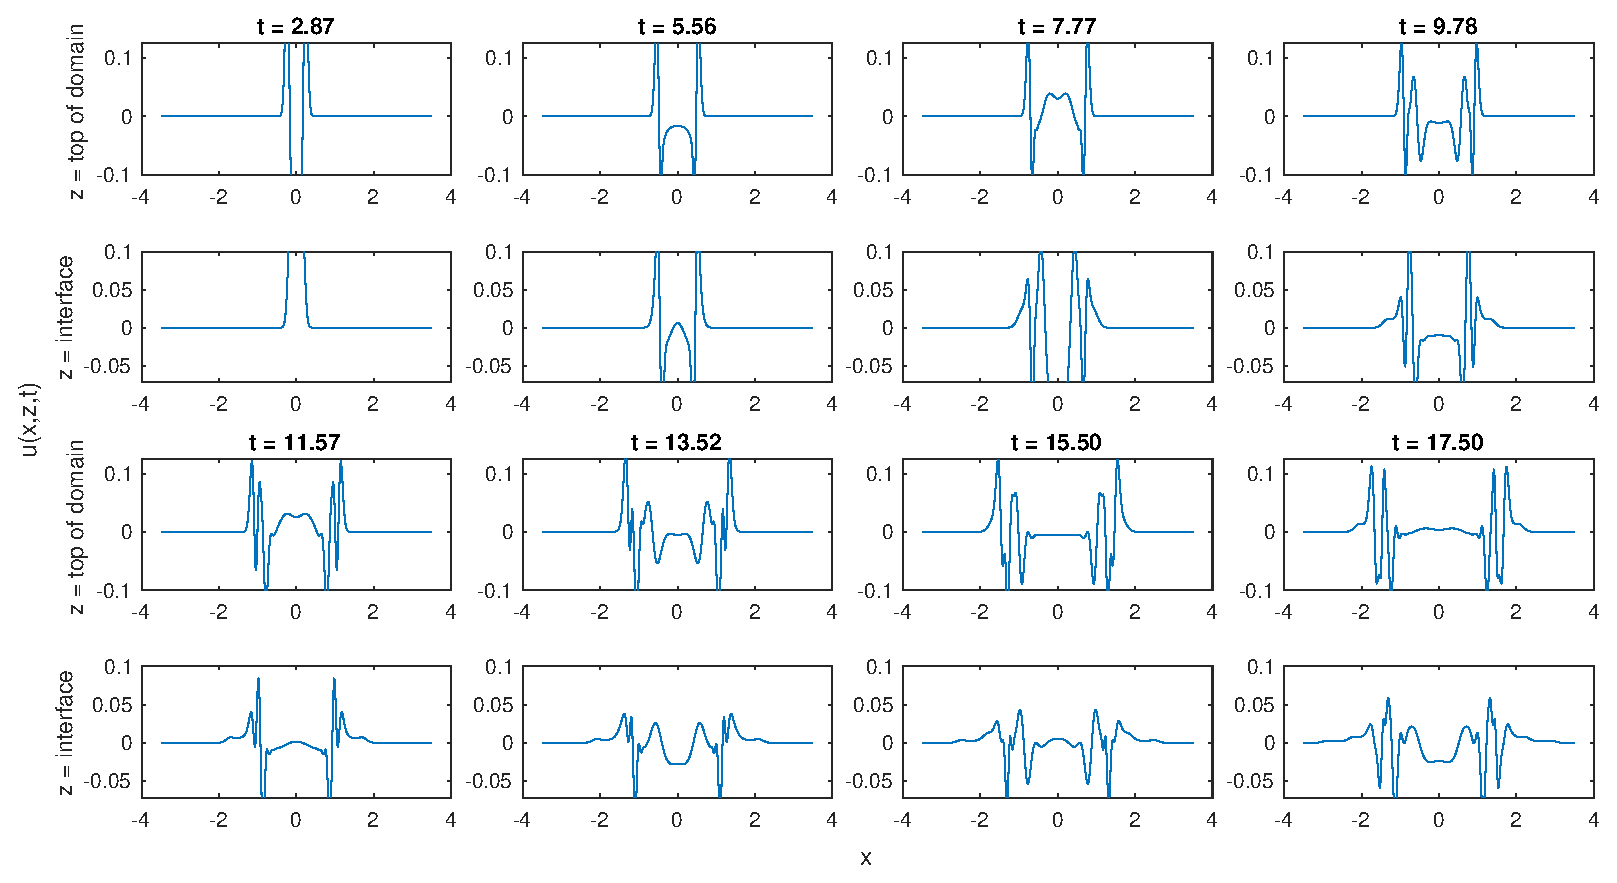
\includegraphics[width=\linewidth]{figures/gaussian_above_c1c2/u_inter_boundary}
\footnotesize
\centering

The parameters are $c_1 = 0.1$, $c_2 = 0.2$, $A=1$, $H=0.5$, and $h = 0.02$. \textcolor{orange}{from Shawn: I don't think the 1D waves are insightful in this case}
\end{figure}

\begin{figure}[htbp]
	\caption{Speed of $u$ along the interface and boundary from Figure \ref{fig:gaussian_above_c1c2}}
	\label{fig:gaussian_above_c1c2_speed}
	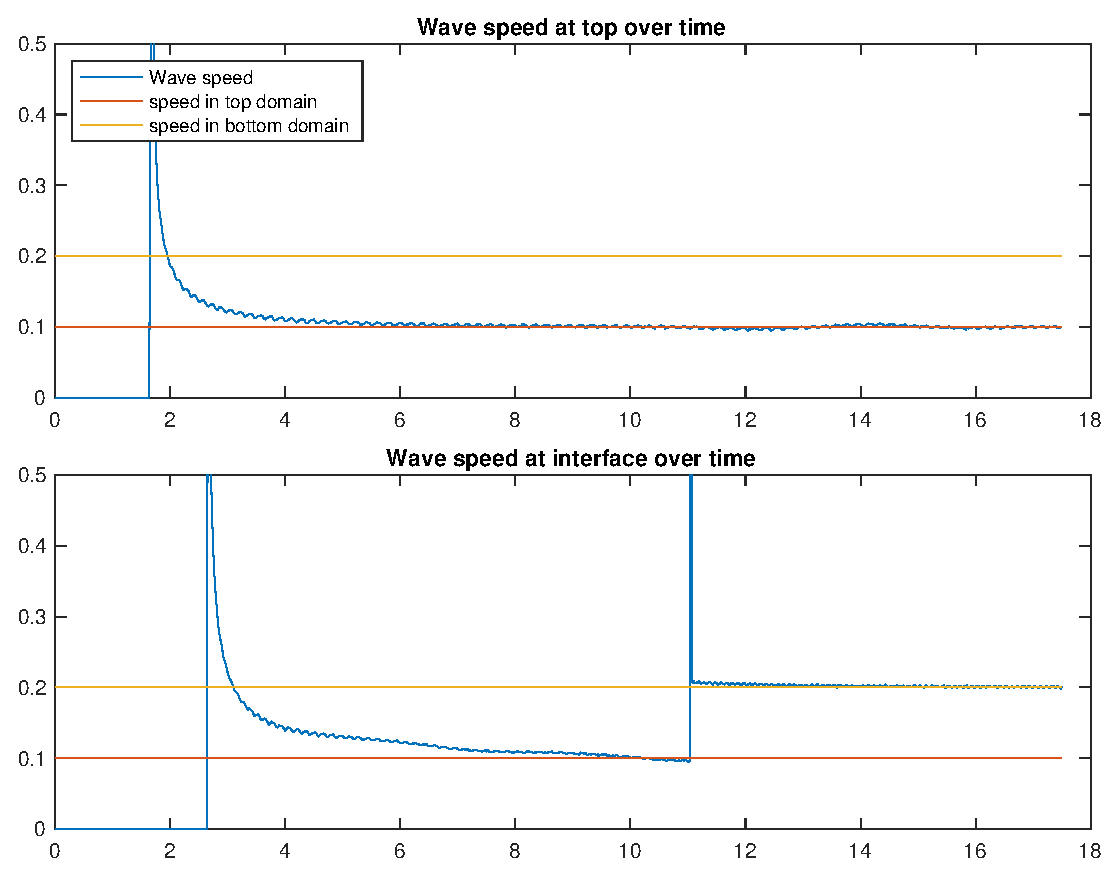
\includegraphics[width=\linewidth]{figures/gaussian_above_c1c2/wavespeeds}
\footnotesize
\centering

The outermost wave at the interface suddenly moves at speed $c_2$ around $t=11$ because that is when the initial wave is overtaken by a shock wave from the top.
\end{figure}


\begin{figure}[htbp]
	\caption{Plots of $u(x,z,t)$ with $c_1>c_2$ after a Gaussian explosion centered in the lower half-space}
	\label{fig:gaussian_below_c2c1}
	\includegraphics[width=\linewidth]{figures/gaussian_below_c2c1/overhead}
	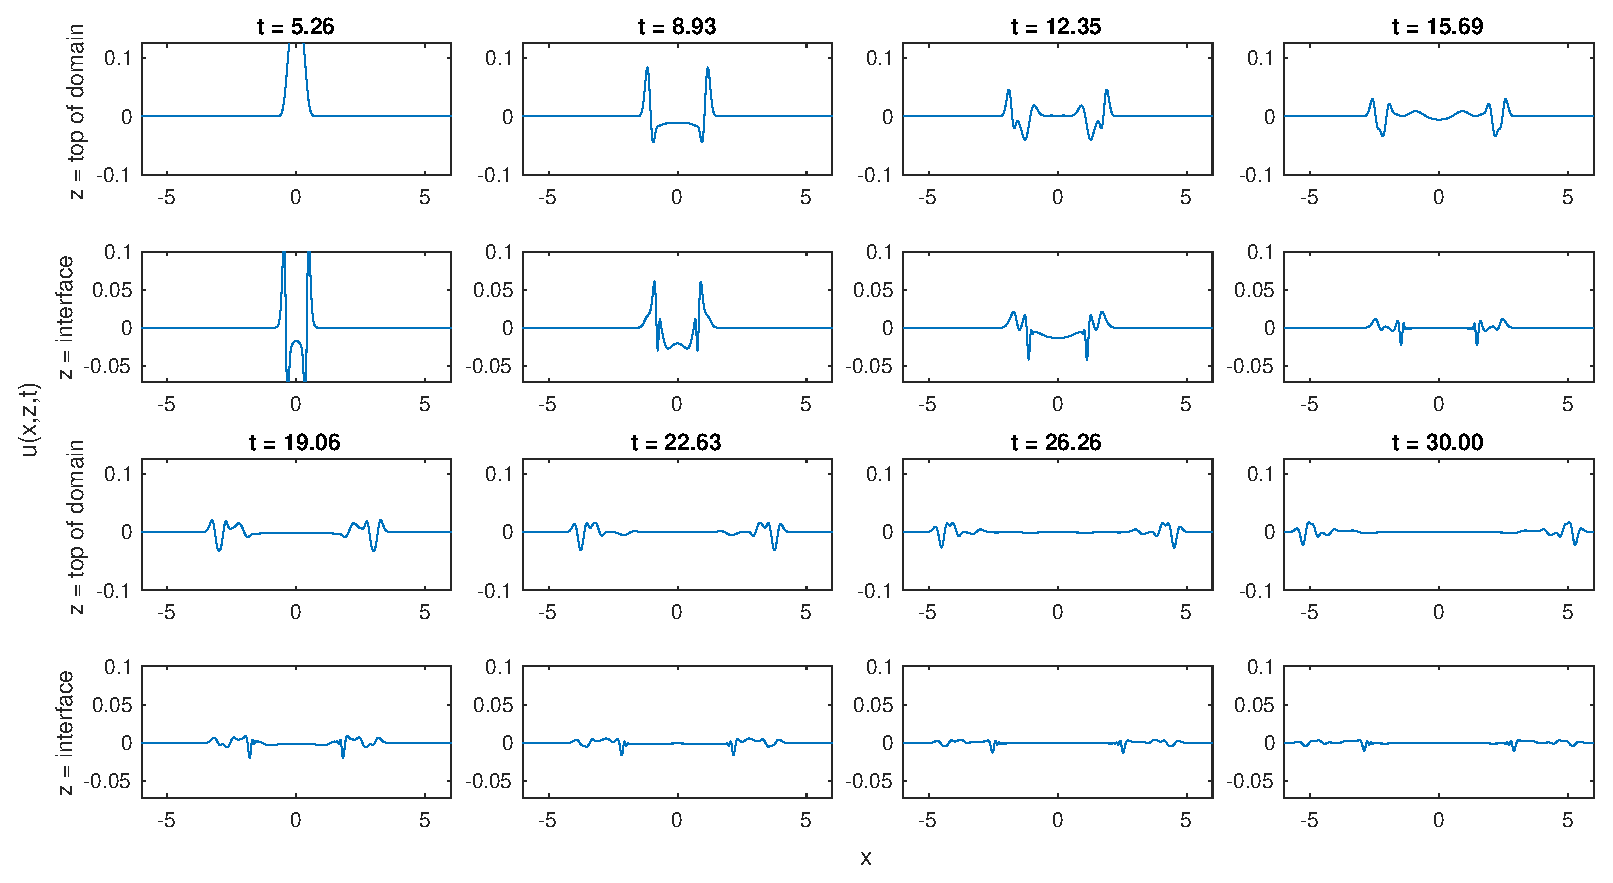
\includegraphics[width=\linewidth]{figures/gaussian_below_c2c1/u_inter_boundary}
\footnotesize
\centering

The parameters are $c_1 = 0.2$, $c_2 = 0.1$, $A=1$, $H=0.5$, and $h = 0.02$.
\end{figure}

\begin{figure}[htbp]
	\caption{Speed of $u$ along the interface and boundary from Figure \ref{fig:gaussian_below_c2c1}}
	\label{fig:gaussian_below_c2c1_speed}
	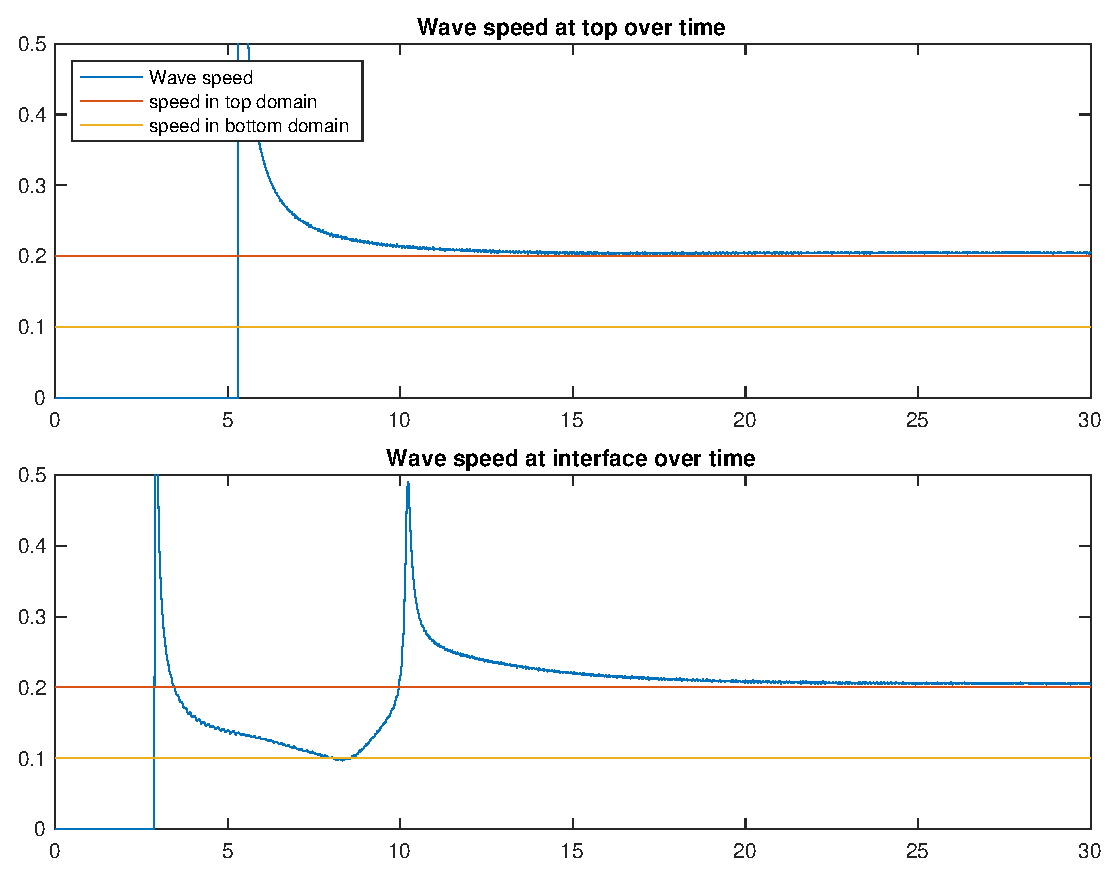
\includegraphics[width=\linewidth]{figures/gaussian_below_c2c1/wavespeeds}
\footnotesize
\centering

\end{figure}


\begin{figure}[htbp]
	\caption{Plots of $u(x,z,t)$ with $c_1>c_2$ after a Gaussian explosion centered in the upper layer}
	\label{fig:gaussian_above_c2c1}
	\includegraphics[width=\linewidth]{figures/gaussian_above_c2c1/overhead}
	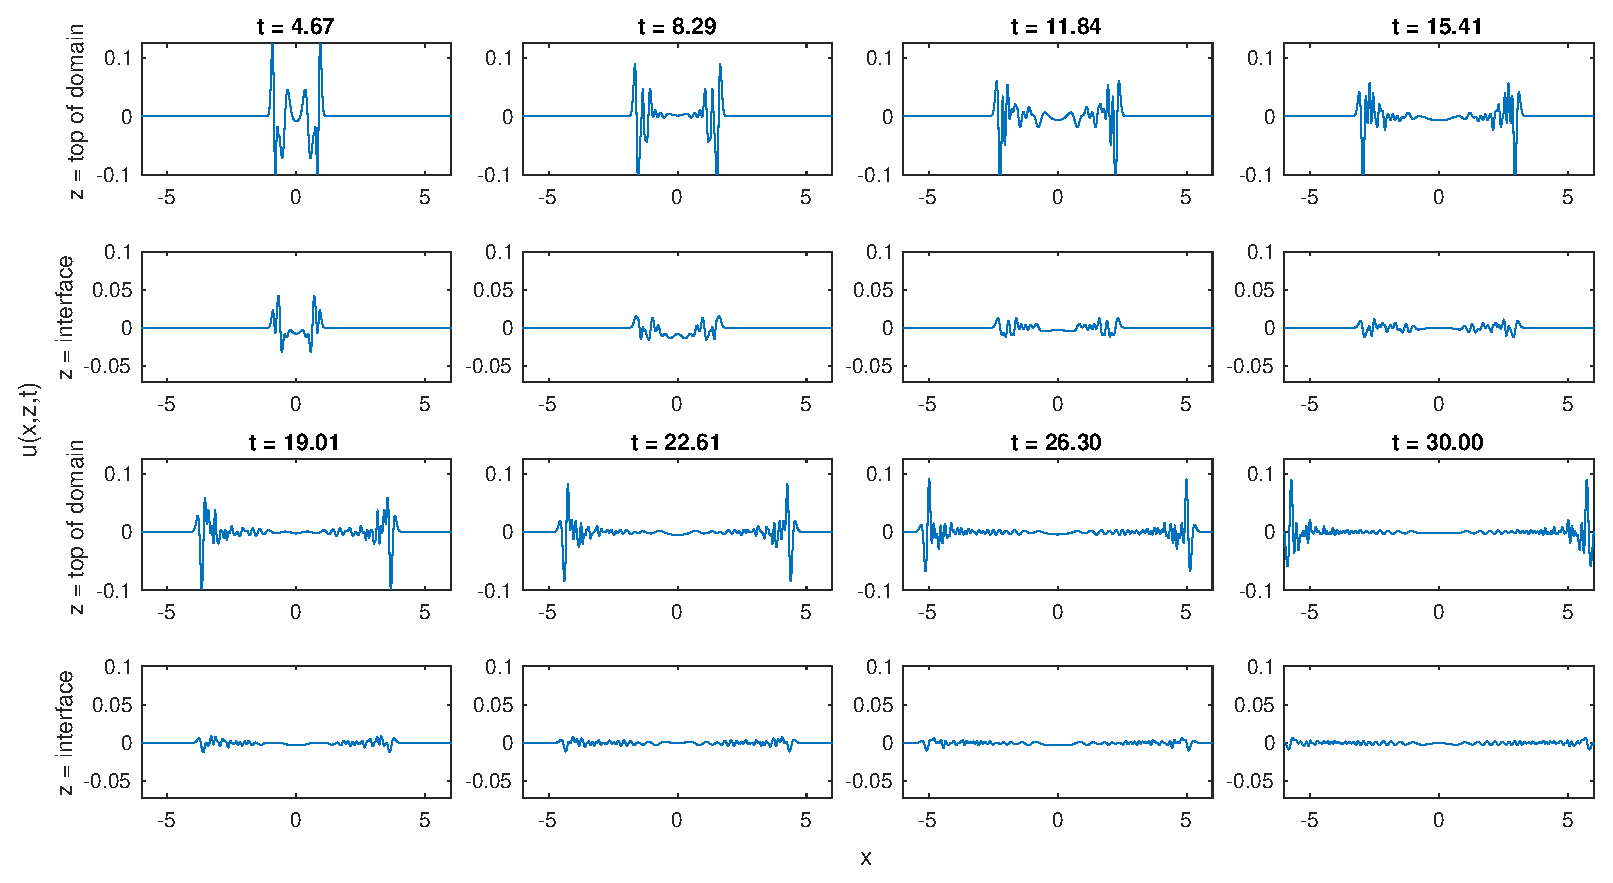
\includegraphics[width=\linewidth]{figures/gaussian_above_c2c1/u_inter_boundary}
\footnotesize
\centering

The parameters are $c_1 = 0.2$, $c_2 = 0.1$, $A=1$, $H=0.5$, and $h = 0.02$.
\end{figure}

\begin{figure}[htbp]
	\caption{Speed of $u$ along the interface and boundary from Figure \ref{fig:gaussian_above_c2c1}}
	\label{fig:gaussian_above_c2c1_speed}
	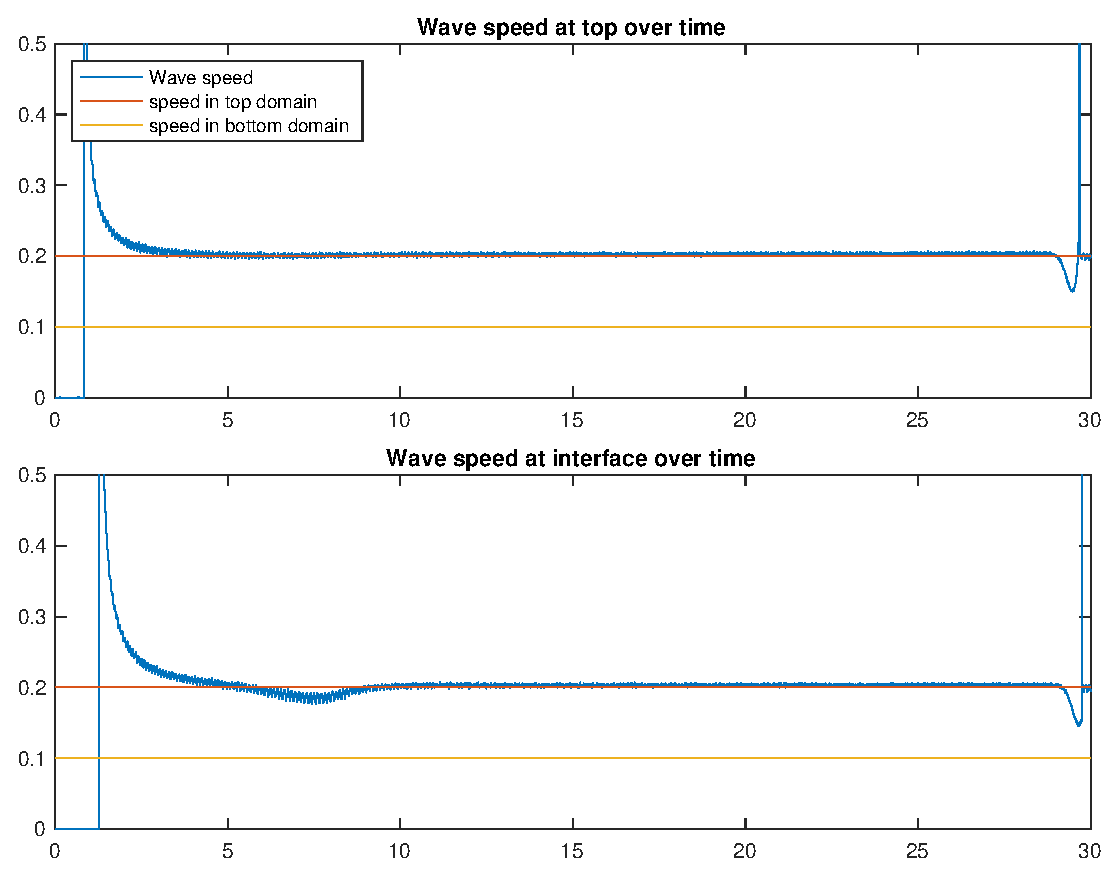
\includegraphics[width=\linewidth]{figures/gaussian_above_c2c1/wavespeeds}
\footnotesize
\centering

\end{figure}



\section{Discussion}\label{sec:Discussion}

**************************Discussion*********************************************

Mention: new models provide better approx than linear Love when linearization is not possible: larger displacements, like mechanical vibrations of human organs near the source, or motion of geological formations near the focus of the earthquake **** Also to Intro!***


Mention future: anisotropic materials, fiber families (C Lee and JF/StJ research)


\subsection*{Acknowledgements}

S.A. thanks the Department of Mathematics and Statistics, University of Saskatchewan, for the support throughout the Master's thesis program. A.C. is grateful to NSERC of Canada for research support through a Discovery grant.

{\footnotesize
%\bibliography{CLN_waves_biblio21}
\bibliography{SA_AS_bib_03}
\bibliographystyle{ieeetr}
}




\end{document}




